% Design Document
% CS 461 - CS Senior Capstone
% Fall 2017
% Authors: Connor Christensen, Lily Shellhammer, William Buffum

\documentclass[draftclsnofoot,onecolumn,letterpaper,10pt]{IEEEtran}

% Packaging
\usepackage{geometry}
\usepackage{hyperref}
\usepackage{titling}
\usepackage{color}
\usepackage{listings}
\usepackage{cite}
\usepackage{pdfpages}
\usepackage{pdflscape}
\usepackage{url}
\usepackage{array}
\usepackage{xargs}                      % Use more than one optional parameter in a new commands
\usepackage{enumitem}
\usepackage{graphicx}
\usepackage{subcaption}
\usepackage{float}
\usepackage{longtable}
\usepackage{standalone}

\setcounter{tocdepth}{4}
\setcounter{secnumdepth}{4}

\geometry{letterpaper, margin=.75in}

% Title page
\title{CS 463 - CS Senior Capstone
	\\Spring 2017
	\\Final Report
}


\author{
	Connor I. Christensen \\
	\texttt{chriconn@oregonstate.edu}
	\\
	Lily M. Shellhammer \\
	\texttt{shellhal@oregonstate.edu}
	\\
	William B. Buffum \\
	\texttt{buffumw@oregonstate.edu}
}

\begin{document}

\begin{titlingpage}
    \maketitle
    \begin{abstract}
			This document details the design and documentation of the Ninkasi Brewhops capstone project.
			Ninkasi Brewing Company is based in Eugene, Oregon, producing and distributing nearly 100,000 barrels of beer each year across the United States and Canada.
			Up until this point, Ninkasi was tracking brewery data using digital and paper spreadsheets.
			Our captone team, comprised of Oregon State Computer Science seniors Connor Christensen, Lily Shellhammer and William Buffum, created a web app for database mangaement to streamline Ninkasi's data collection and tracking.
			We created a database connected to a website for entering fermentation measurements, checking tank statuses, and viewing data over time.
			Our goal is for our site to prevent the errors and delays digital spreadsheet tracking caused.
			The beta version of our site has been delivered to Ninkasi for testing.
			\\
			\textbf{Keywords: Brewing, Operation, Management, Ninkasi, Oregon State University}
    \end{abstract}
		\pagebreak
		\tableofcontents
\end{titlingpage}

\section{Introduction}
	\subsection{Who requested it?}
	Daniel Sharp, Director of Operations, at Ninkasi Brewing Company requested this system.

	\subsection{Why was it requested?}
	Over the last ten years, Ninkasi Brewing Company has exploded in growth.
	With their growth came an influx of data.
	Previously, brewers would manually check all the tanks, write down data points on paper, and transfer those values to an Excel spreadsheet.
	The spreadsheet was then sent around to every individual who needed the values.
	There are several issues with this method: human error, not efficient, and data isn't seen in a timely fashion.
	As Ninkasi continues to grow, these issues will continue to grow.

	\subsection{What is its importance?}
	If Ninkasi cannot maintain consistent batches of beer, then their market share will suffer.

	\subsection{Who was your client?}
	Our client was Daniel Sharp, the Director of Operations at Ninkasi Brewing Company.

	\subsection{Who are the members of your team?}
	The members of our team include: Lily Shellhammer, Connor Christensen, and William Buffum.

	\subsection{What were their roles?}
	Lily Shellhammer was in charge of connecting the client side application to the server side.
	Connor Christensen was in charge of the front end web design.
	William Buffum was in charge of the backend REST API and the database where information is stored.

	\subsection{What was the role of the client?}
	The client helped the development team understand all the business needs of the application.
	Daniel helped us solidify a database structure and gave input on the frontend design.
	
\section{Requirements Document}
	\subsection{Original Document}
	\subsubsection{Introduction}
	\paragraph{Purpose}
		This document will outline a project that satisfies the requirements for Ninkasi's new brewing operations data management system.
		This includes a detailed description of the product created and the technology utilized to build the product.
		This document is intended for a technical audience, primarily for our instructors, Kirsten Winters and Kevin McGrath, and our sponsor, Daniel Sharp.

	\paragraph{Scope}

		This project is to develop a web application and relational database model to manage Ninkasi's data.
		We will perform a cost-benefit analysis to recommend hosting the system with web service provider versus hosting on Ninkasi servers.
		The database\footnote{Details on database information are outlined in section 3.4} will store all information that is required during the brewing process.
        This information is pulled directly from the Master Excel Spreadsheet that Ninkasi uses to track brewing process data.
        \\
        \\
		The provided interface will allow brewers to manually insert new batch records, update incorrect data, and view existing data.
		The web application interface will allow Ninkasi personnel to view basic status information on tanks at a glance.
		We will gage adequacy of interface based on a minimum 60\% approval from Ninkasi personnel, of which Daniel Sharp must approve.
		The goal of these requirements is to stop use of Excel as primary data storage.
		\\
		\\
		Stretch goals are outlined in section 3.2.
		\\
		\\
		We are not be responsible for advanced application security or direct control of any brewing process.

	\paragraph{Definitions, Acronyms and Abbreviations}

    \begin{itemize}
      \item Database - area in system where collected information will be stored
      \item Cellaring data - data collected by our database; data collected while cellaring beers
      \item Data points - information to be stored in our database\footnote{Breakdown of all data points found in section 3.4}
      \item BrewHops - The name of our team
      \item BOMS - Brewery Operations Management System
      \item Master Excel Spreadsheet - Ninkasi currently tracks all data using a spreadsheet, referred to as the "Master Excel Spreadsheet"
    \end{itemize}

	\paragraph{Overview}
		In the next sections, this document outlines details on the hardware, software, and user interface requirements for our project.
		It explains what needs to be completed in order to launch our minimum viable product.
		Security, functionality, and organization are explained in detail.

\subsubsection{Description}
	\paragraph{Product Perspective}
		\textbf{System interfaces}

			Brewers will interact with our web application in the cellar.
			The web application interacts with the database and will enter data points from the brewer's entry into the form.
			If we meet our stretch goals, brewers will be able to extract Excel spreadsheets from our web application.

		\textbf{User interfaces}

			The user will interact with the web application through either an internet connected phone, tablet, desktop, or laptop computer.
			Phones will operate almost exclusively in portrait mode.
			Apart from the occasional chart or data display, most of the use for the phone will be entering data, which benefits from a portrait layout.
			Tablets have the ability to use both portrait or landscape mode, depending on how they would like to use the device, and which method is more convenient for them.
			Desktops and laptops will work in a landscape mode.
			For big enough screens, extra space can be used to fit more functionality on one page without having to hide menu items or actions, such as extracting data from the database.
			\\
			\\
			All Ninkasi brewers use a company provided phone and most of the brewer's work will be done through that phone.
			It's important that the site be consistent between iOS and Android to increase reliability, allow brewers to help each other with problems regardless of operating system, and reduce the learning curve.
			The environment in which the brewers are working requires that the data entry system be clear, easy to see, and have a forgiving\footnote{Error handling to prevent incorrect information from being added to the database. Will require Daniel Sharp's approval to be considered adequate.} interface.
			For any new hires, the system should be intuitive\footnote{60\% acceptance of interface required to be considered "intuitive"}.
			Some phones may have smaller screens or may be held at a distance, so it's important that the font be big enough, the contrast strong enough, and the input boxes take up as much space as they can so they are easy to tap and input is easy to see.
			Brewers may have water, grain dust or other materials on their hands that will interfere with the touch capabilities of the device.
			Making the interface forgiving by making buttons, input fields and any other interactive components large will reduce error and frustration.
			\\
			\\
			The system should use terminology that brewers are familiar with.
			Reports should be color coded to keep the screen from filling with text and to allow brewers access to data easily\footnote{60\% approval from brewers will be considered "easily" accessible data}.

		\textbf{Hardware interfaces}

			Ninkasi has a small server in their headquarters.
			A cost-benefit analysis will determine if this server will satisfy the hardware requirements of the system.
			If it will not, we will provide at least one recommendation for web service providers.

		\textbf{Software interfaces}

			The user will interact with data via a web application.
			The application will expose input forms to submit data.
			We will release the software in stages, starting with a database, then a basic web input form connected to the database, then our final minimum viable product will include the data display interface.
			The data display interface will involve giving basic information about the status of the tanks in the facility, and which actions the brewers should take to make sure that the product will be developed properly.
			Streatch goals include more advanced data display such as the ability to show simple graphs of data over time for any tank.

		\textbf{Communications interfaces}

			Web application will not implement other interfaces.

		\textbf{Memory constraints}

			Currently Ninkasi has space on a single server in a back room.
			If Ninkasi's storage requirements grow quickly, a single server may not meet the needs of our system.
			If Ninkasi decides to host our database on a 3rd party cloud hosting site, the memory constraints will be those of how much space they buy.

		\textbf{Site adaptation requirements}

			Brewers will adapt to using our web form rather than continue implementing the system they previously used.
			They will enter data only through the web application.

	\paragraph{Product functions}
		Product includes the development of a relational database and development of a web application to process and present database information.
		Brewers will input information to the database using a form on the website.

	\paragraph{User characteristics}
		Brewers using the web application will have all levels of education, including PhD, MS, BS, and little to no college experience.
		Their technical expertise about web development and coding in general will be minimal, but they will understand how to use mobile applications, how to access websites, and how to enter data into forms.

	\paragraph{Constraints}
		\textbf{Regulatory policies}

		Because we are creating this software from the ground up and there are no previous regulations for a system like this, this section is not applicable for the BrewHops team.

		\textbf{Hardware limitations}

		Ninkasi has a small server that we may utilize for the database.
		If we decide not to use a third party hosting site, then the small server means there will only be the amount of free space on the server available.
		This is a not a limitation for our project so much as a limitation for any possible continuation of our project from Ninkasi.

		\textbf{Interfaces to other applications}

		BrewHops’ application will integrate with Tanknet.
		\footnote{Tanknet is a a hardware and software system that performs physical measurements of brewing vats and automatically collects the data and exports it digitally}
		The web application will automatically collect temperature information from Tanknet and store it in our database.

		\textbf{Parallel operation}

        Our web application will allow concurrent read access and use transactions for insertions and updates.

		\textbf{Audit functions}

        The system will store past data\footnote{Past data stored as far back as deemed necessary by Daniel Sharp, or within limitations of server space.} to be used for audit functionality.

		\textbf{Control functions}

        Not applicable for BrewHops team.

		\textbf{Higher-order language requirements}

        Objects and callback functionality may be necessary.

		\textbf{Signal handshake protocols (e.g., XON-XOFF, ACK-NACK)}

        BrewHops team will not work directly with handshake protocols, these protocols will be abstracted by the technologies used.

		\textbf{Reliability requirements}

		The web application will ensure data integrity for automated data collection.
		The web application will validate data entered manually.
		Our site will be accessible without wait time longer than 5 seconds 90\% of the time\footnote{This may vary depending on the hardware capabilities of Ninkasi servers.}.

		\textbf{Criticality of the application}

		The web application is not critical to Ninkasi Brewing Company’s success, but it will save the company data entry time.
		Ninkasi already has a working system that is not online.
		Our system will improve the current system by reducing time wasted from data entry error and replace their working data entry processes.

		\textbf{Safety and security considerations.}

		This product will be light on security, as it is an internal application and should only be accessed by verified employees in the company.
		As this is not a public facing product, malicious activity is low on our list of priorities.
		Further details are outlined under the Specific Requirements section.

	\paragraph{Assumptions and dependencies}
    BrewHops team will have access to Ninkasi Brewing Company's server to deploy application.
    Ninkasi is willing to use the software technologies and languages we develop in.

\subsubsection{Specific requirements}
	\paragraph{External interfaces}
    Included in product are as follows:
        \begin{itemize}
				\item{Database: A database will either be hosted on Ninkasi's server or through a 3rd party site.
                The input to the database will include multiple columns of cellaring data, who entered the information, and timestamps. }

            \item{Web Application:}
            The web application will consist of a website that scales/changes functionality to fit the device.

                \begin{itemize}
				    \item{Mobile Phone Page: The web application will scale to fit the mobile phone, mostly in portrait mode.
					The mobile version will be used for data entry and will have minimal options in comparison with the tablet or desktop.}

                    \item{Tablet Page: Tablets will operate in either portrait or landscape mode and will have the form and possibly more options for data extraction.}

                    \item{Desktop/Laptop Computer Page: This page will operate in landscape mode and will have the most options of the three pages.}

                \end{itemize}
        \end{itemize}

	\paragraph{Functions}

		Data will be validated upon input to database.
		Information being entered that is far outside the range of expected values will prompt the user to verify that the information is indeed correct.
		Every input form will strip out all html special characters to make sure that no harmful code can be injected into the database.

		Stretch goals include:
		\begin{itemize}
			\item{Adding a login interface to verify the users before they begin using the system.}

            \item{Implement profile levels to differentiate permissions (admin, operator, supervisor, cellar, etc.).}

            \item{Track authenticated user levels in database.}

			\item{Including a time and ID stamp on the data entered in case the company needs to trace back an error to a particular time or person.}
		\end{itemize}

	\paragraph{Performance requirements}
		Multiple users on the web application at once will be permitted.
        Application should not crash if multiple brewers input data at the same time.
		95\% of interactions with the web page should happen in less than 20 seconds\footnote{This assumes basic interactions and prior experience with the system.}.

	\paragraph{Logical database requirements}
    \begin{itemize}
        \item{Information pulled from Master Excel Spreadsheet}
            \begin{itemize}
                \item{\textbf{Fermentation Vessel, FV}:
                    tank fermentation is carried out in.
                }
                \item{\textbf{BEER}:
                    beer abbreviations associated with temperature profiles and dry hop recipes.
                }
                \item{\textbf{BATCH}:
                    batches are groupings of sequential brew numbers inside a particular FV\footnote{Example: if there are 5 brews of IPA with numbers 3000, 3001, 3002, 3003, and 3004 in FV7, the BATCH ID will be: IPA 3000-3005 FV7.}
                }
                \item{\textbf{Yeast Generation, GEN}:
				    the generation of the yeast we use to ferment the beer.
                }
                \item{\textbf{Vol To Ferm (BBL)}}
                \item{\textbf{Vol To Bright (BBL)}}
                \item{\textbf{BRIGHT (BRITE)}:
                    tank where beer is sent after fermentation, used to track volume of beer and associated losses.
                }
                \item{\textbf{\% Yield}:
                    normally stored onces per batch but a batch from one FV may split between two smaller brite tanks or two batches from two FVs may blend into single brite tank.
                }
                \item{\textbf{Dry Hop/Amount Type}:
                    recipe for given dry hop
                    \footnote{Example: dry hop type A = 50 lb, dry hop type B = 75 lb.}
                    \footnote{Dependent on the BEER and volume in fermentation (for dry hops).}.
                }
                \item{\textbf{Amount (lb)}:
                    amount in lbs of dry hops to be added to tank.
                }
                \item{\textbf{Monitoring Points}:
                    minimally measured daily.
                }
                \begin{itemize}
                    \item{\textbf{Specific Gravity}:
                        A measure that represents the amount of sugar left in the beer.
                        This number starts high and decreases throughtout fermentation.
                        When it stops we move on to the next process step
                    }
                    \item{\textbf{pH}:
                        pH level of batch in brewing vat.
                    }
                    \item{\textbf{ABV}: Alcohol By Volumne of batch.}
                    \item{\textbf{Temp}: Temperature of batch.}
                    \item{\textbf{Action}: Action taken.}
                    \item{\textbf{By}:
                        person taking the action above.
                    }
                \end{itemize}
            \end{itemize}
        \item{Frequency of use}

            Data currently updated daily and read throughout the day.

        \item{Accessing Capabilities}

            Database will be access from database access layer of web application.
    \end{itemize}

	\paragraph{Design constraints}
		Ninkasi currently has one server.
		Our job is to create, or aid in creating, a new database system.
		We can either use their existing platforms, meaning limited space, or create a database on a third party hosting site.
		Either option is limited by time, we can only implement so much of the data management throughout the timeline of this project.
		Stretch goals are to expand the database and data entry options, given we have time to do so.

		\textbf{Standards compliance}

		The database will store information with correct relationships according to Ninkasi's current Master Excel Spreadsheet.

	\paragraph{Software system attributes}
		\textbf{Reliability}

		There is room for occasional bugs given that they do not damage data or inhibit the brewery process.
		Reliability of the system is a desirable goal, but the product is not a mission critical piece of software.
		Down time would be frustrating for employees, but would not render the company useless.
        A stretch requirement will be that the system is active or available 96\% of the time\footnote{Measuring this will depend on if the system is deployed for at least 30 days before the Spring term expo showcase.}.

		\textbf{Availability}

		The system should not require a reboot, recovery or restart after deployment.
		Stretch goals include making a daily backup of the information in the database if the system were to crash or the data were to be corrupted.

		\textbf{Security}

		Individuals not associated with Ninkasi Brewing Company should not have access to the system.
		As this is not a public facing product, malicious activity is low on our list of priorities.
		Stretch goals will focus on security such as providing a login interface for employees, adding time stamps for data entered, and providing an easy method to find out who was responsible for entering incorrect data or misuse of the system.
		There will be checks built into the delivered product, but those will primarily be designed for taking care of user error rather than malicious intent.

		\textbf{Maintainability}

		This software is designed to be a proof of concept that having a system like this would be beneficial to Ninkasi's business development.
		Therefore, maintainability is not only good as a good coding practice, but it is one of the core requirements for the project that the code be maintainable and well documented\footnote{Documentation will be stored in the GitHub repository.}.
		\\ \\
		There should be a clear separation between the frontend and the database connections.
        This may be done through a REST API structure.
        This would allow future developers to implement new interfaces as needed.
		\\ \\
		For the most part, code should be broken up into discrete functions that would allow for unit testing in the future.
		Though unit testing is not required as a goal for this project, the ability to attach some kind of testing framework will be useful.

		\textbf{Portability}

		This program is designed to be highly portable and the format of the product was selected specifically for that reason.
		The percentage of code and components with host-dependent elements should be as small as possible, likely around 40\%.
		Our site will be built using web technologies that will operate properly on Chrome and Firefox.
        In order for the system to function properly, the hosting server must have the technologies used in the system, installed.

	\paragraph{Organizing the specific requirements}
		We will build a user class based system.
        This will allow us to separate responsibilities and functionality so individuals only have access to their required tasks.
        In this system, we can design it hierarchically so that managers have access to all data manipulation privileges while brewers only have read or write privileges through structured forms.
        As a stretch goal, manager level individuals will be able to modify user permissions as needed.

\pagebreak
\includepdf[pages=1-2]{OSUNinkasiCapstone.pdf}

	\subsection{Modifications}
	The only modifications that were made to the Requirements Document over the course of the year was to remove some sections that were not applicable to our project such as which handshake protocols our project would use.
	\subsection{Updated Gantt Chart}
	\includepdf[pages=1]{OSUNinkasiCapstoneFinal.pdf}
\section{Design Document}
	\subsection{Original Document}
	% Design Document
% CS 461 - CS Senior Capstone
% Fall 2017
% Authors: Connor Christensen, Lily Shellhammer, William Buffum

\documentclass[draftclsnofoot,onecolumn,letterpaper,10pt]{IEEEtran}

% Packaging
\usepackage{geometry}
\usepackage{hyperref}
\usepackage{titling}
\usepackage{color}
\usepackage{listings}
\usepackage{cite}
\usepackage{pdfpages}
\usepackage{pdflscape}
\usepackage{url}
\usepackage{array}
\usepackage{xargs}                      % Use more than one optional parameter in a new commands
\usepackage{enumitem}
\usepackage{graphicx}
\usepackage{subcaption}
\usepackage{float}
\usepackage{longtable}

\graphicspath{ {images/mobile/} }
\graphicspath{ {images/stack/} }

% Type of paper
\geometry{letterpaper, margin=.75in}

\begin{document}


\section{Overview}
	\subsection{Scope}

	Our project seeks to provide a more user-friendly method for Ninkasi to interact with its brewery data.
	This will increase efficiency and product consistency, while decreasing the amount of manual labor for the brewers.

	\subsection{Purpose}

	This document will discuss which components require more intensive design decisions to be made, and how to approach these categories in a way that will make the development process easier and more reliable.
	Multiple revisions of this document will ensure that the development process will be reasonable for the developers while still meeting all the goals that the client has outlined.

	\subsection{Intended audience}

	The primary audience for this document is the client.
	The document is also aimed towards those that wish to gain a more technical explanation about how the BrewHops team will approach the project.

\section{Definitions}
\begin{longtable}{p{4cm}p{12cm}}
    Host & The hardware the database is hosted on \\
    Platform & The application that the database will run on \\
    Database & The program that stores and retrieves the information \\
    Database Interaction Language & The langauage that serves as the middle man between the database and the front end. It makes requests to the database and processes those requests to send the smallest and most organized form of the information it can to the front end. \\
    Styling & The look of the website \\
    Interactive Web Framework & A package of code that allows for easy manipulation of the content and look of the page without having to refresh the page or interact with the server. \\
    Client & Daniel Sharp, Ninkasi Brewmaster \\
    BrewHops & Name of the development team \\
    Cellaring Data & Data of the beers fermenting in the cellar \\
    Specific Gravity & Measurement that represents the amount of sugar left in the beer. This number decreases throughout fermentation and is inversely related to alcohol content. \\
    ABV & Alcohol by Volume \\
    Brand & Name of the beer associated with the recipe \\
    Generation & Generation of yeast used to ferment \\
    Volume to Ferment & Volume of beer going into the fermentation process \\
    CRUD & Create, Read, Update, Delete \\
    GET & A method of getting information through the URL \\
    POST & A method of sending information from a website to a server \\
    PUT & Sends information to a specific server and if something is already there, it will overwrite it. \\
    PATCH & Sends information to a location and updates what is there \\
    DELETE & Deletes information on the server it makes the request to \\
    Routes & A method of creating specific paths in the URL where the website can make requests to get or modify data from the server. \\
    API & Application Program Interface: A method for designing how a piece of software or user can interact with a program \\
    REST & REpresentational State Transfer: A design pattern for web development that utilizes an API for all interactions between servers and web clients. \\
    Server side processing & Code that is run on the server \\
\end{longtable}

\section{Design}
	\subsection{Introduction}
	This document will outline the design decisions made on
	\begin{itemize}
		\item database structure
		\item REST API
		\item general user interface
		\item mobile user interface
		\item maintainability
	\end{itemize}

	\begin{figure}[H]
    \centering
    \begin{subfigure}[b]{0.2\textwidth}
        
\includegraphics[height=5cm]{images/stack/abstract}
        \caption{The most abstract version of the site. This is separated into the front and back end. The back end code, represented in blue, runs on the server. The front end code, represented in green, runs on the tablet, phone, laptop or desktop that the user is operating.}
        \label{fig:abstract}
    \end{subfigure}
    ~
    \begin{subfigure}[b]{0.2\textwidth}
        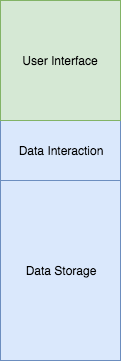
\includegraphics[height=5cm]{images/stack/abstract_medium}
        \caption{The abstract model with more concrete definitions of the location where the data is stored, the layer that serves as the interaction point between the two, and the interface.}
        \label{fig:abstract_medium}
    \end{subfigure}
    ~
    \begin{subfigure}[b]{0.2\textwidth}
        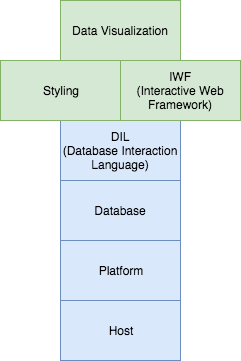
\includegraphics[height=5cm]{images/stack/general_tech}
        \caption{The same stack showing how each component breaks down into the technologies listed in the tech review. All sections on the middle right stack are summarized in the definitions section. }
        \label{fig:general_tech}
    \end{subfigure}
		~
    \begin{subfigure}[b]{0.2\textwidth}
        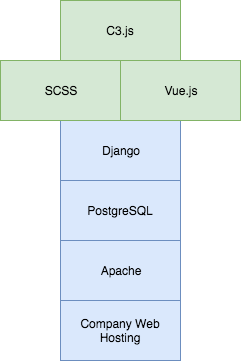
\includegraphics[height=5cm]{images/stack/chosen_tech}
        \caption{The full stack with the technologies BrewHops has selected for the project.}
        \label{fig:chosen_tech}
    \end{subfigure}
    \caption{The web tech stack with varying levels of specificity}\label{fig:animals}
		\end{figure}


	\subsection{Viewpoints}

		\subsubsection{Database Structure}

		The main purpose of our project is to bridge the gap between Brewers and the database at Ninkasi. Designing a functional database is key to making this project a success.
		Our database needs to connect the cellaring data on each beer for each day it is measured.
		The beers need to be connected to their predefined recipes.
		As brewers make decisions on what steps to complete next, the database needs to show what steps have already been completed via the information previously entered.
		It needs to keep track of who entered what data and whether the information entered is within the acceptable measurement ranges.

		The database system is based off of the excel spreadsheet currently in use by Ninkasi for storing data.
		Each beer is connected to a predefined recipe, and each beer currently in the cellar is associated with data collected each day, along with the alerts in place for that day.
		Our database design has 5 tables: TankActions, TankContents, TankInfo, BrandInfo, and Employees.
		Employees contains login usernames, passwords, and ID numbers for the employees.
		This is used for the login system and also for keeping track of who entered the TankContents information.
		The BrandInfo table keeps track of a brand’s recipe and the ranges associated with correct values.
		This is so that we can alert the brewers if temperature, gravity or pH are outside of the typical or safe levels.
		The last three tables are associated with the tanks, what’s inside of them, and the measurements of the beer in each tank.
		The TankInfo table contains TankID, beer name, batch number, generation, and volume to ferment.
		Each tank can have 1 or more TankContents, as each TankContent data set is taken on a different day and a batch can be in a tank for multiple weeks.
		TankContents contain the date on which the measurements took place, specific gravity, pH, ABV, temperature, and the EmployeeID who entered the data.
		TankActions hold actions that need to happen, the date, the TankID they are associated with, and the EmployeeID who satisfied the action, if they have fixed the problem.

		This system works for our project because it allows us to keep track of:

		\begin{itemize}
			\item What brand and batch are in each tank
			\item What is happening in that tank every day
			\item What actions need to be taken, and if they have been taken care of
			\item Who entered the data
			\item What the correct measurement ranges and ingredients are for each brand
		\end{itemize}

		\begin{itemize}
			\item Issues brought up:
			\item Inefficient query system if you want batch information over long periods of time
			\item BRITE is not anywhere in our diagram and the team is unsure where it belongs in the data structure
			\item Recipie is not a long varchar in the database
		\end{itemize}

		\subsubsection{RESTful API}

		Ninkasi needs all CRUD operations available to their user interfaces.
		To adhere with these standards, the API must be fully RESTful and expose the necessary GET, POST, PUT, PATCH, and DELETE routes.
		The API will have direct access into the database and will need to be secured per user so that only individuals with adequate permissions have access to certain API routing features.
		Other security concerns are that individuals outside of Ninkasi do not have access to the API.
		This will not be the BrewHops team’s primary concern as Ninkasi network security should handle these concerns when application is deployed.


		The user interfaces for the data management system need efficient access to all information stored in the database.
		The interfaces need to be able to get the data, insert new data, update old data, and delete incorrect data.
		Each route of the REST API will give access to these operations based on the type of operation performed on the url.

		Interfaces will need access to all information in the TankInfo table.
		To allow this, the routes on the /tanks url will handle retrieving all Tanks data, inserting and updating Tanks data, and retrieving batch information for each tank.

		What follows are each route and their purpose in the API:

		/api/tanks:
		\begin{itemize}
			\item GET: (queries TankInfo database table to get)
			\begin{itemize}
				\item TankID
				\item BrandID
				\item BATCH
				\item Yeast Generation
				\item Ferm\_To\_Vol
			\end{itemize}
			\item POST: (add a new Fermentation Tank to the database)
			\item /:id:
			\begin{itemize}
				\item GET: Query TankInfo for all batches produced in Tank
				\item POST: Add new batch to tank
				\item :id/:id\_batch: \\
					GET:
					\begin{itemize}
						\item Gets all rows of TankContent for BatchID
						\item PUT: update entire batch resource
						\item PATCH: update part of a batch resource
						\item DELETE: destroy a batch resource
					\end{itemize}
				\end{itemize}
		\end{itemize}


		The user interfaces also need access to the Employees table in the database to authenticate users and regulate permission capabilities of various users.
		To do this, we expose a /users route on the url that allows the interfaces to pull back information on all users or specific users.
		/api/users:
		\begin{itemize}
			\item GET: get a list of all users from Employee table
			\item POST: add user to Employee table

			\item /:id
			\begin{itemize}
				\item GET: get a user resource
				\item PUT: update entire user resource
				\item PATCH: update part of user resource
				\item DELETE: destroy user resource
			\end{itemize}
		\end{itemize}


		Our user interfaces may also need access to brand information on different beers.
		To facilitate these needs, we expose a /brand route on the url to access all brands or specific brands stored in the BrandInfo table.

		/api/brand:
		\begin{itemize}
			\item GET: retrieve list of all Ninkasi brands from BrandInfo
			\item POST: add a new brand

			\item /:id
			\begin{itemize}
				\item GET: retrieve all brand information
				\begin{itemize}
					\item Recipe
					\item List of batch ids currently in progress
				\end{itemize}
				\item PUT: update entire brand resource
				\item PATCH: partial update of brand resource
				\item DELETE: delete brand resource
			\end{itemize}
		\end{itemize}


		A RESTful API is important because it improves application maintainability and testability.
		Maintainability is a primary concern and requirement of this project.
		Ease of testing ensures the integrity of our final product and gives us further metrics to gage success.
		A REST API allows the BrewHops team to fully decouple\footnote{“decouple” means separate user interface concerns from server-side processing concerns} user interfaces from the backend processes.
		This is important because development on the user interface and the server-side support can work in parallel; the only dependency is how data is structured.
		Once data structure is determined for each route, our frontend developer can mock data\footnote{mocking data means to create a static data source for testing purposes} to test the interface while our backend developer builds out each route to the specifications.
		RESTful APIs also improve application testability by allowing developers to leverage testing frameworks designed for specific technologies.

		\subsubsection{General User Interface}

		The user interface needs to be designed in a way that is easily usable by the brewers.
		The UI design decisions will first be made by the BrewHops team.
		A prototype of the UI will be developed by the team based on the goals outlined by the client.
		The user interface will then go through an iterative feedback process where the client will provide changes, the team will revise the document and make new suggestions, which will then be returned to the client.
		This process will continue until both parties have verified that the design is both achievable by the development team and meets the goals of the client.
		Iterative design ensures that there is a balance of input, with multiple opportunities for everyone to contribute to the project.
		The BrewHops team has design experience, and it will be best for them to make a majority of the decisions about how the user interface will function.
		This will keep the burden of development off of the client, while still giving them an option to weigh in on changes they see being beneficial to their operations.

		\subsubsection{Mobile User Interface}

		The interface designed must be capable of running on both a large screen desktop and a mobile device.
		Basic data display and entry functionality must exist on mobile devices to meet project specifications.
		The process for designing the mobile interface will be the same iterative design process as the general interface.
		A mockup for mobile design shown in the appendix.
		This is the first form of the interface, and over the course of building the application, frequent feedback from the client will be taken into account to ensure that all goals are met in a way that works well for the client.
		Rationale for the mobile design is the same as that of the general user interface.

		\subsubsection{Maintainability}

		After we leave this project, Ninkasi needs other developers to be able to maintain our code and improve upon it.
		The most important thing is leaving good documentation in the project.
		This design document, along with the other papers written for the senior capstone course should serve as a good starting point.
		While the code is being written for the project, documentation on the code itself and its organizational structure should be used.
		Every folder with custom code in it should have a markdown document describing the contents of the documents.
		Assistance in locating code will come with use of common programming languages and design patterns.
		For example, ruby on rails is a popular web framework that comes with a base template.
		Common structures such as these are familiar to many programmers and should keep the project from being too difficult to interpret for new developers.
		Open source projects have been struggling with ensuing that contributors know how to read the code that exists in the project, and write changes that are useful to the project.
		There has been a development of general design strategies used in the open source community to ensure a maintainable project, and utilizing these strategies will create a project that will be maintainable for whoever works on the project after the BrewHops team is done.


		\section{Appendix}
		\subsection{Mobile Design}
		\centering
		\begin{tabular}{ll}
				Home & Menu \\
				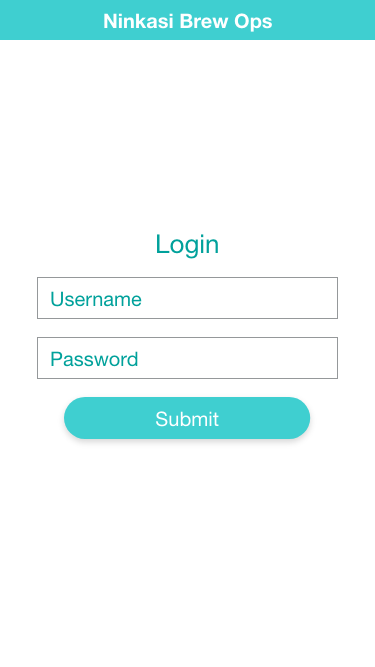
\includegraphics[scale=.3]{images/mobile/home} & 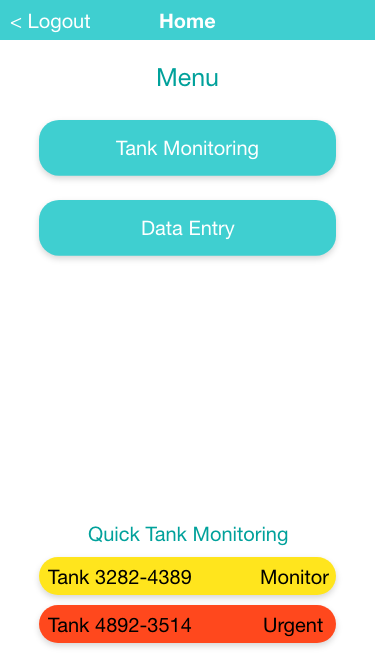
\includegraphics[scale=.3]{images/mobile/menu} \\
				Data Entry & Confirmation Page \\
				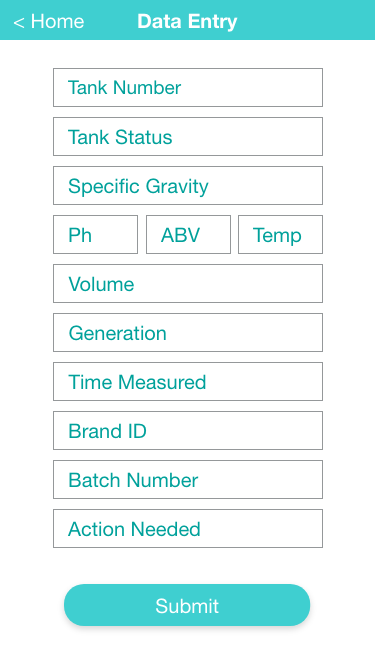
\includegraphics[scale=.3]{images/mobile/data_entry} & 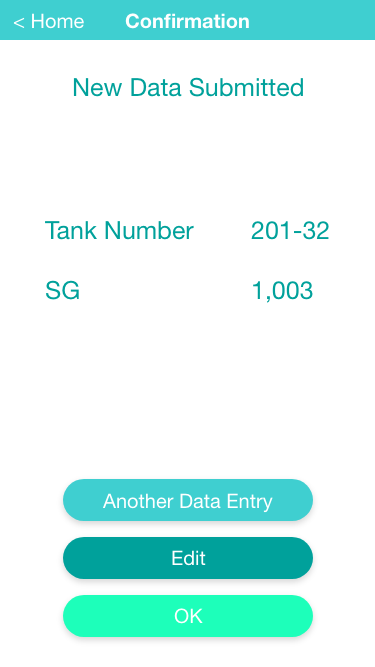
\includegraphics[scale=.3]{images/mobile/confirmation_page} \\
				Tank Monitoring & Tank Info \\
				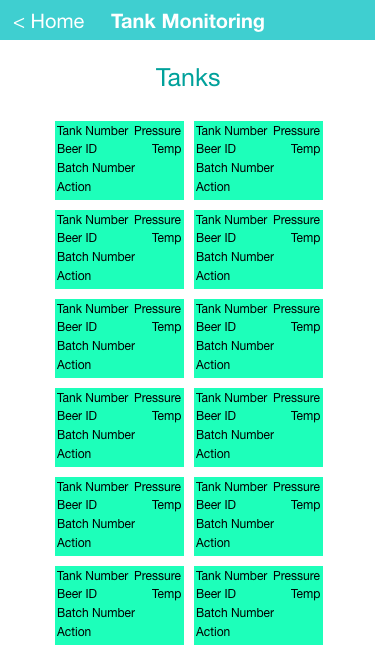
\includegraphics[scale=.3]{images/mobile/tank_monitoring} & 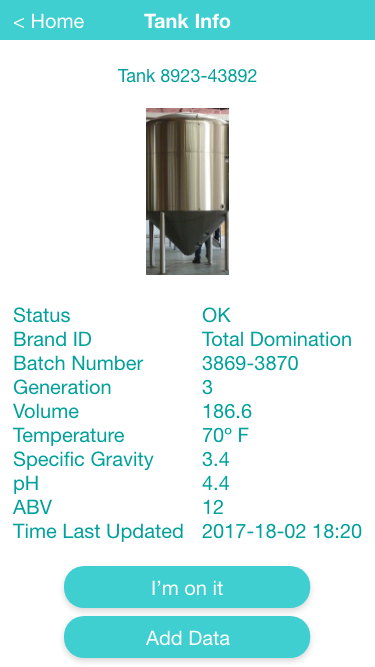
\includegraphics[scale=.3]{images/mobile/tank_info} \\
		\end{tabular}

		\subsection{Desktop Design}
		\begin{tabular}{l}
				Admin \\
				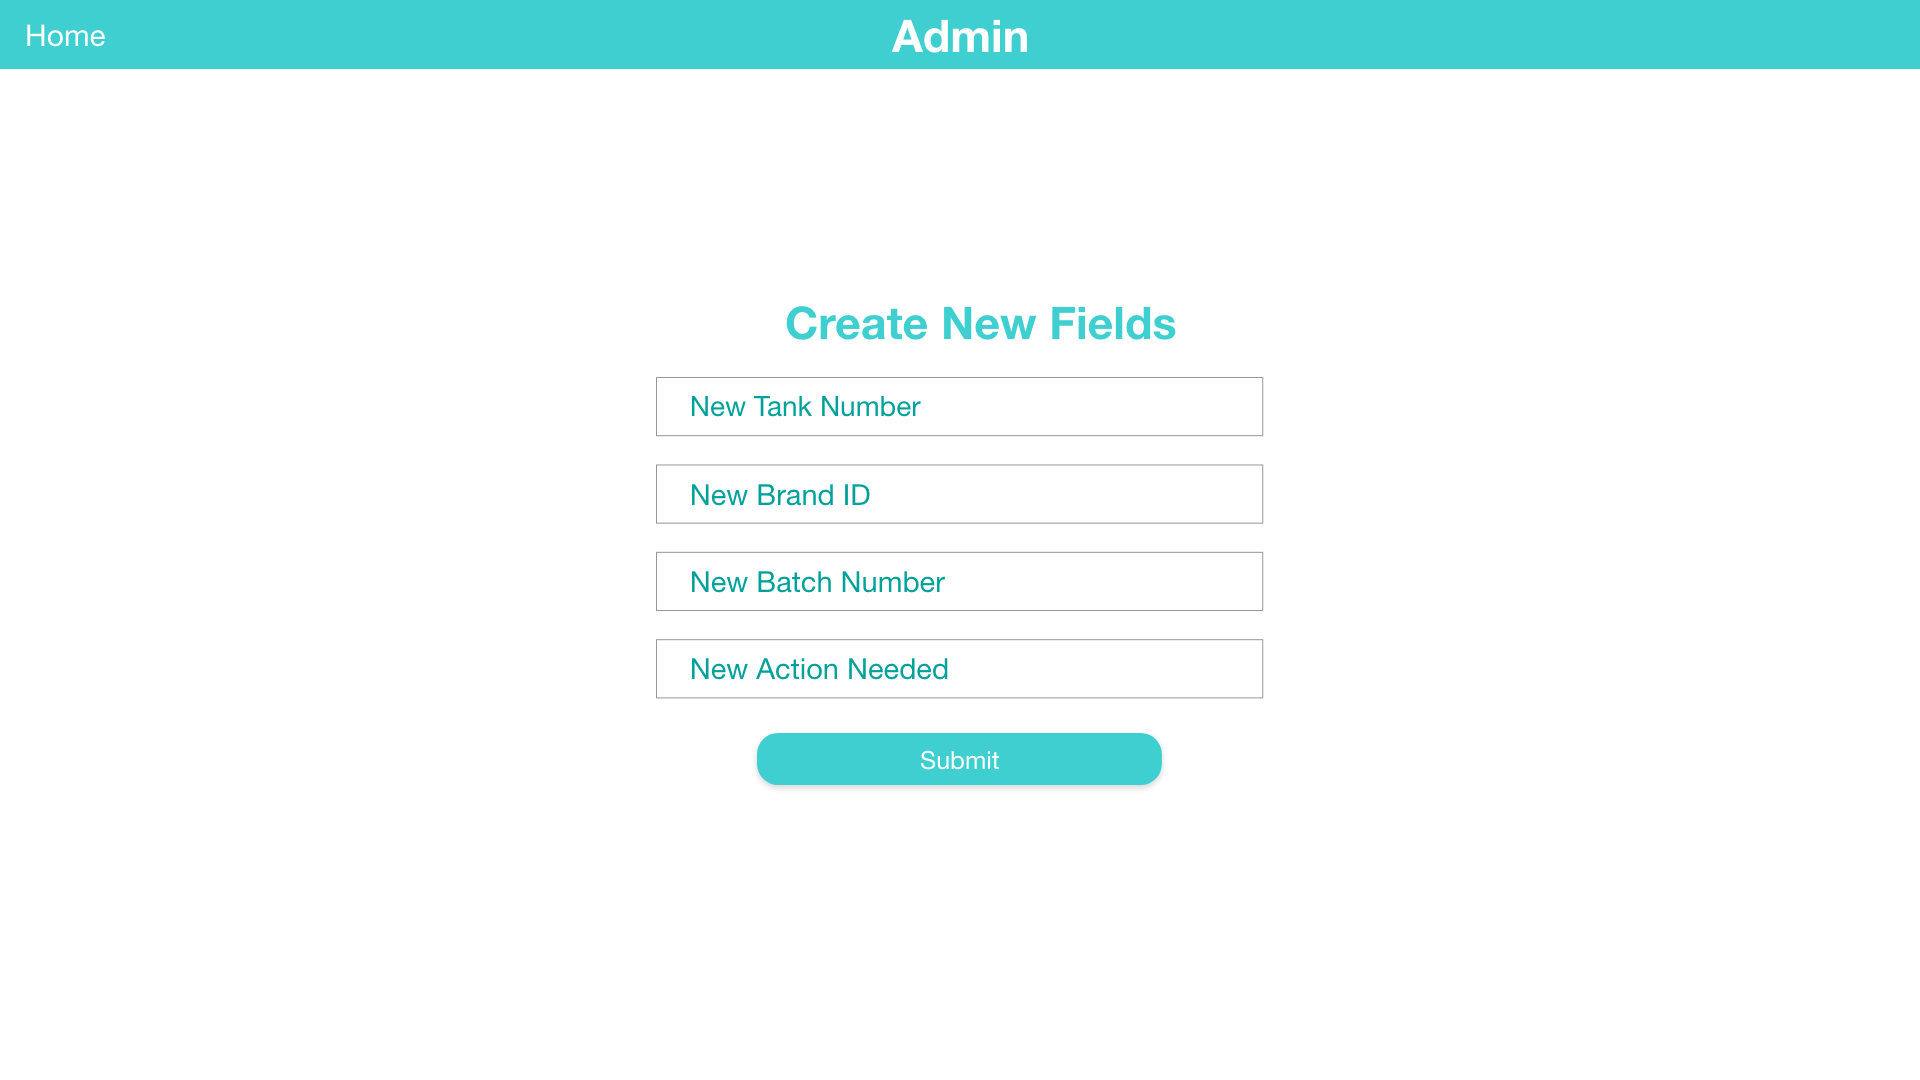
\includegraphics[scale=.15]{images/web/admin} \\
				Home \\
				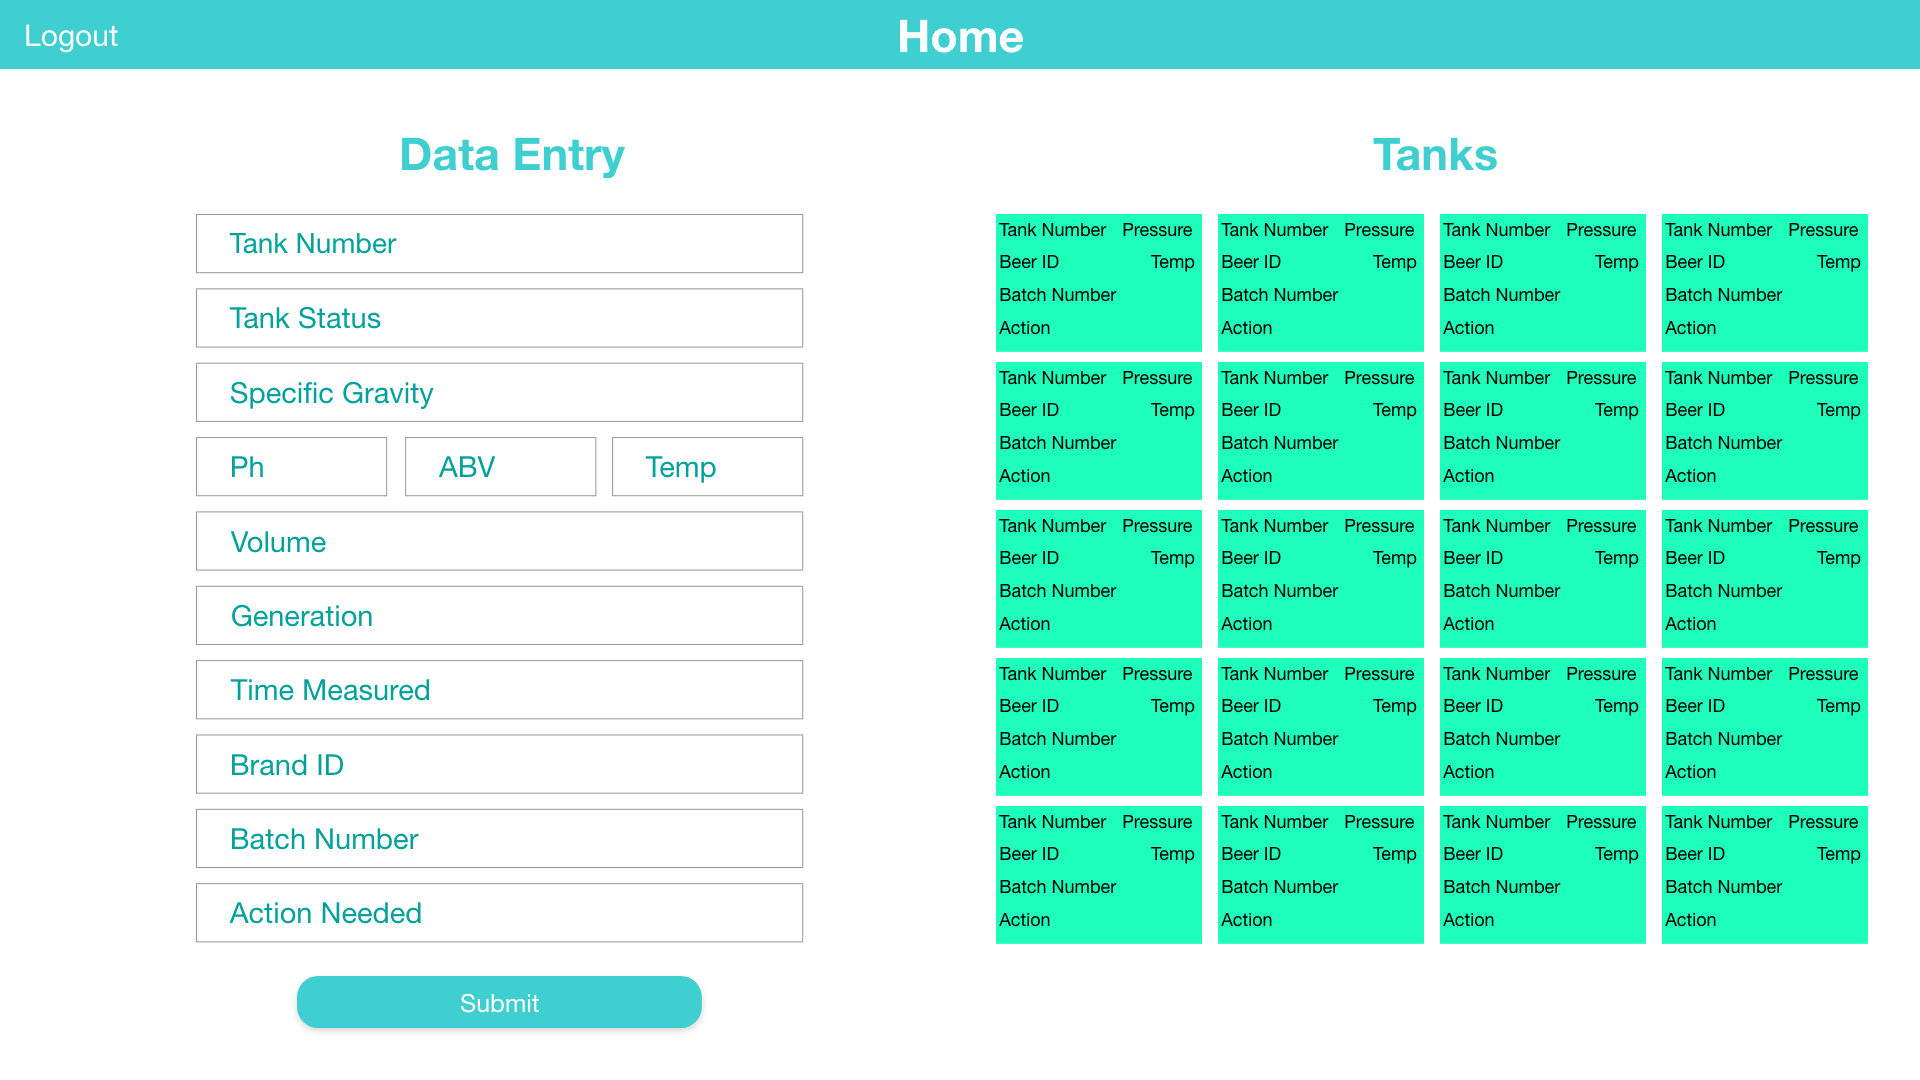
\includegraphics[scale=.15]{images/web/home} \\
				Login \\
				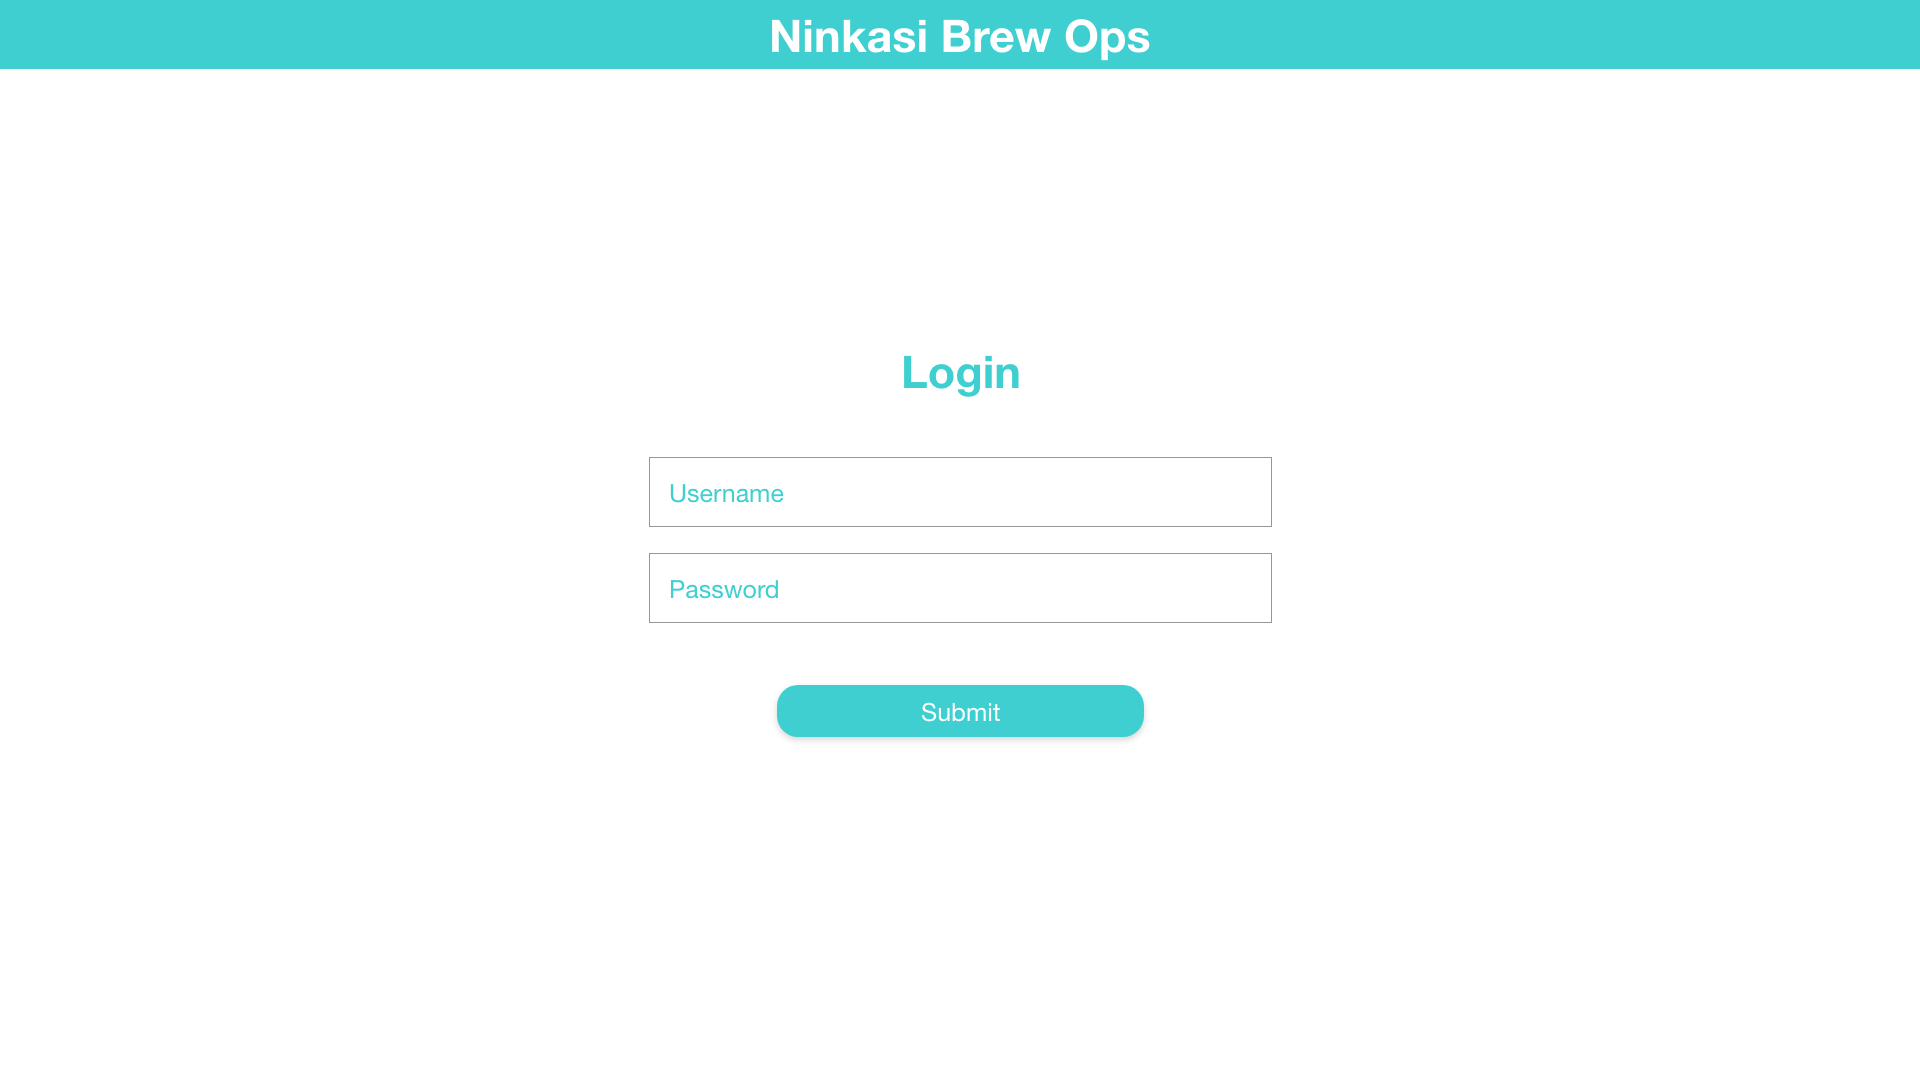
\includegraphics[scale=.15]{images/web/login} \\
				Tank Info \\
				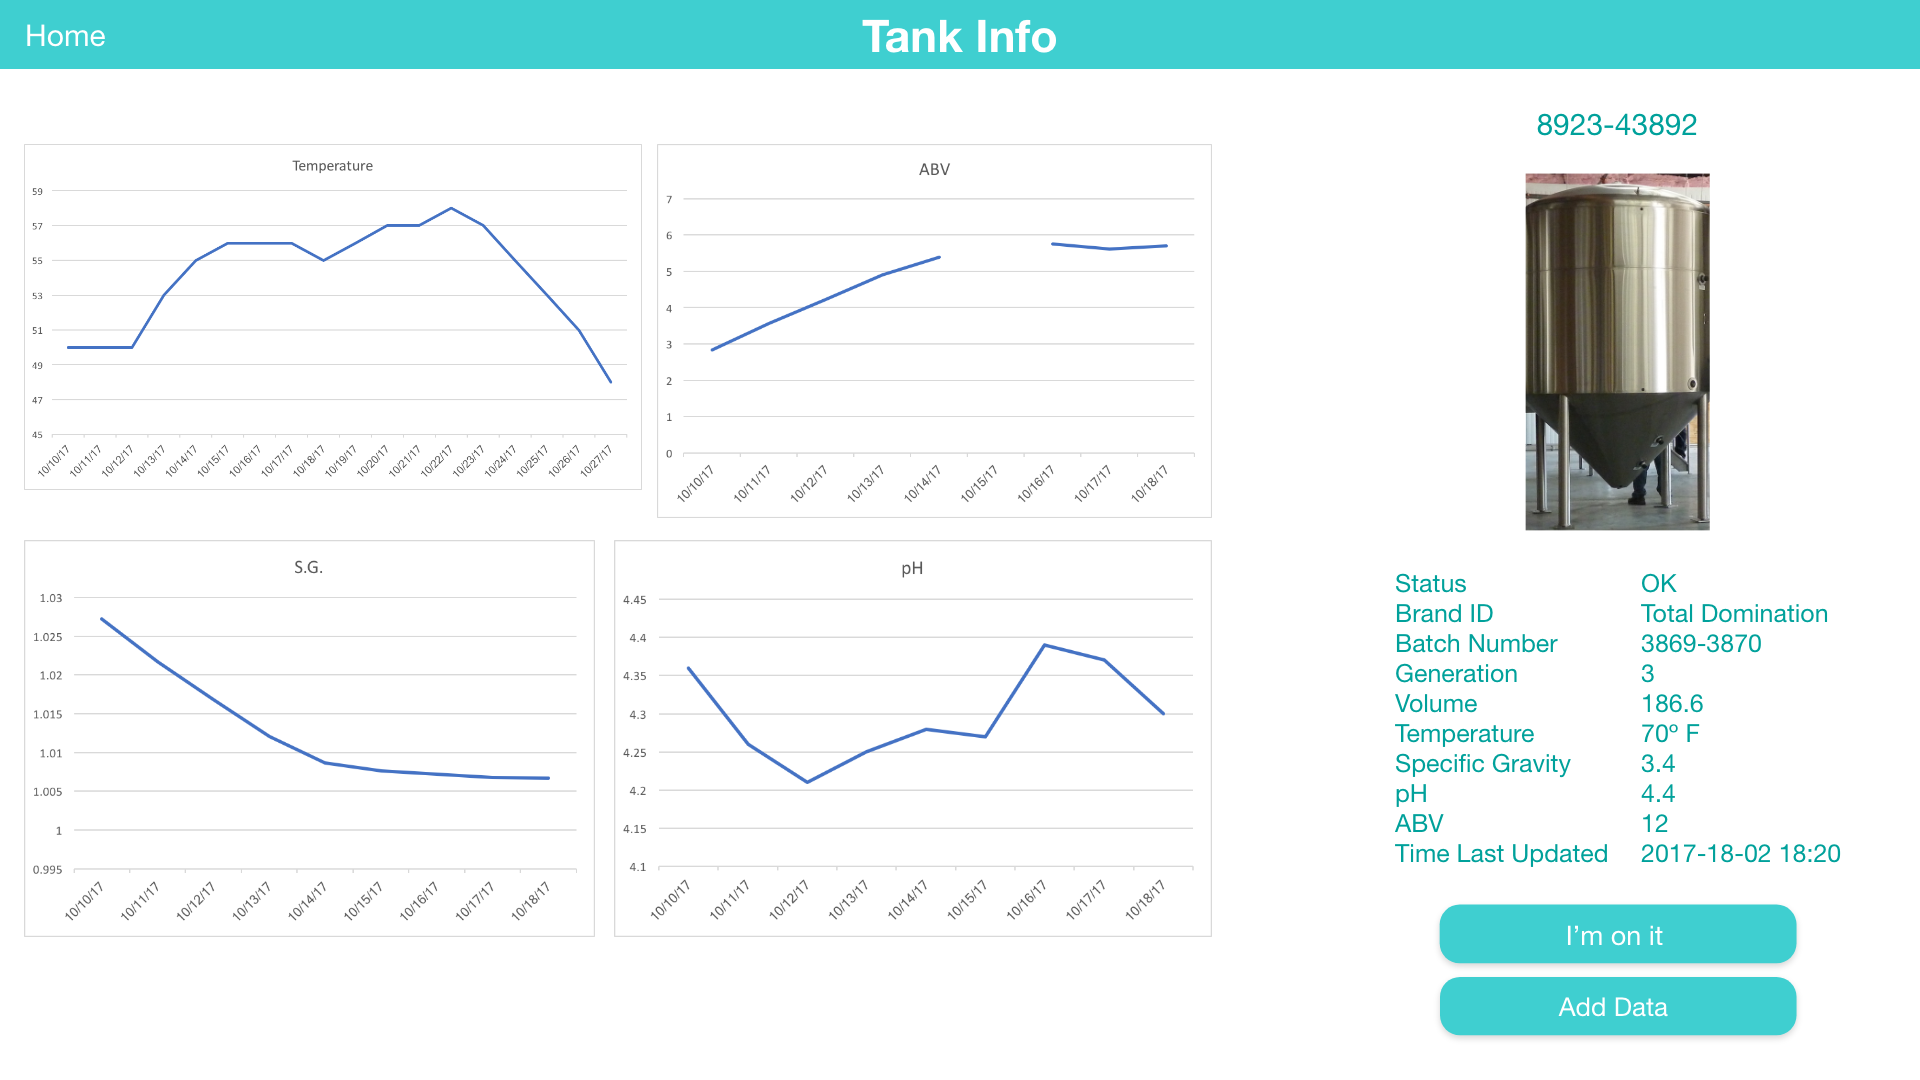
\includegraphics[scale=.15]{images/web/tank_info} \\
		\end{tabular}

\end{document}

	\subsection{Modifications}
	While the structure of our stack is similar, we have changed some of our technologies.
	We are using Ruby on Rails as our server side langugage instead of Django.
	Our database also has a different layout that works better for rotating batches in tanks.
	We have 5 tables: tanks, batches, batch contents, actions, and tasks.
	Tanks hold information on each tank.
	Batches are stored in tanks and have multiple batch contents which are taken daily, if not more often.
	Actions holds the list of actions that can be taken on tanks, and tasks assigns actions to certain tanks.

\section{Tech Review}
\subsection{Front-End}
This is a comparison of three front end technologies for web design.
\begin{itemize}
	\item Data visualization seeks to find a framework that will aid in the display of information from the database in a user-friendly way.
	\item Styling attempts to cover available options for creating a nice user interface for the project.
	\item Interactive web frameworks outlines the difference between the major pro's and con's of JavaScript frameworks and whether or not they should be used at all.
\end{itemize}

\textbf{Warning:}
The majority of technologies listed in these categories is open source code that builds off other open source modules.
Including code from other open source projects could potentially lead to legal issues.
Each module added into the project comes with a legal agreement that could potentially cause problems for the company later.
These legal agreements may or may not be enforced and they may or may not conflict with other modules in the project.
It is common web development practice to build frameworks from many sub-utilities and packages that are available in the open source community.
As of yet, there is no dedicated team ensuring that all legal agreements agree with each-other and the requirements of the client, and it is up to the client to decide if they want to take steps to guard against the unlikely event that someone stakes a claim against the company based on those licenses.\\






\subsubsection{Data Visualization}

This is an overview of libraries written for data display in web browsers.
Each of these libraries are built using the web language JavaScript to allow for live interaction with the user.
Table 1 shows the code needed to set up a basic bar graph using each library.
These yield approximately the same visual results.
All have the con that they require JavaScript to be enabled and all of them are open source and free.


\textbf{Critera}


	\begin{itemize}
		\item relatively small amounts of code
		\item stable and consistent in its presentation
		\item provide simple charts and graphs like bar charts and plot point graphs
		\item easy for developers to work with
	\end{itemize}


\textbf{Technology}

	\begin{itemize}

		\item{\textit{D3.js}}


			\textbf{About:}

			D3 stands for Data-Driven Documents and it is a powerhouse of a library for data visualization.\cite{d3.org}
			It was created by a team of PhD graduates working out of the Stanford Visualization Group and is essentially the library for creating amazing data visualization.\cite{d3Journal}
			It has a relatively bulky setup, but allows fine grained detail and control over how data is displayed.
			This library is so powerful that it functions more as a library for painting than for graphing.

			\noindent \textbf{Pros:}

			D3 uses SVG's \footnote{\textbf{S}calable \textbf{V}ector \textbf{G}raphics: A visual component defined mathematically. It can scale up or down to any size without loss of image quality.} which allows it to be able to create any 2d shape that can be mathematically defined.
			SVG's do not require JavaScript to work, though D3 can't run without JavaScript enabled.
			The D3 library uses pre-build JavaScript functions to select elements, create SVG objects, and be able to preform a wide number of transformations on them.\cite{d3.org}
			Transformations are just as precise as the drawing abilities and are limited only by the processing power of the computer and the skill of the programmer.
			It uses jQuery and CSS styled selection and modification of content for flexibility and ease of use.
			Objects that are made with D3 are easily syllable with CSS, meaning that data display can inherit styling rules to maintain a consistent look across the platform.
			D3 has a large community and it was built by very intelligent people early on, so it has only gained in popularity since then.\cite{DataVisProCon}
			The majority of data frameworks are built off of D3.
			As such, there are a huge number of online examples.

			\noindent \textbf{Cons:}

			Despite all its good features, the D3 library adds a lot of code to a project, the learning curve is steep, and the code needed to accomplish a task is verbose.\cite{DataVisProCon}
			The code required to set up a bar graph is massive compared to most other frameworks and the time that it takes to learn D3 is an even bigger obstacle.


		\item{\textit{C3.js}}


			\textbf{About:}

			C3 is a package built off D3 and is formatted specifically for creating graphs.

			\noindent \textbf{Pros:}

			It is beautifully simple to create a graph and plug and play really works in this context.
			It has a great set of examples and documentation is readily available.
			It can easily switch between chart types and display multiple chart types mixed in with a single variable changed in the code.\cite{c3.org}
			The amount of things that just work coming out of C3 is impressive, inclusive of the animations that simply show up whenever you load up a graph.

			\noindent \textbf{Cons:}

			Since it is built off D3, C3 requires D3 to be installed, which causes many lines of code to be added to the project.
			There are nearly 10,000 lines of JavaScript in both D3 and C3, bringing in almost 20,000 lines of code for data display.
			The interface is much easier to use, the tradeoff being more limiting in its expressions.


		\item{\textit{Chart.js}}


			\textbf{About:}
			Chart.js is a JavaScript library that allows you to draw different types of charts using the HTML5 canvas element
			\footnote{HTML Canvas: A new web standard that allows web programmers to create computer graphics created and rendered in the browser.}.

			\noindent \textbf{Pros:}

			Chart.js does not use D3 as its underlying code, which means that it is significantly more lightweight as a package.\cite{ChartJS} Like C3, it is very responsive and the documentation is very good.

			\noindent \textbf{Cons:}

			Use of the canvas comes with a few drawbacks, the most common issue being that it cannot scale without loss of quality.
			The HTML5 Canvas specification recommends that authors should not use the canvas element when they have other more suitable means available.\cite{CanvasVsSVG}
			Canvas is good for 3d graphics, but this ability is not beneficial if you simply want a bar graph.
			If you are drawing little details all very close together, canvas is great for that.
			Canvas is not very accessible as it is just drawing pixels and no data can be extracted by assistive technology or bots.

	\end{itemize}



	\textbf{Conclusion}
	It is on our recommendation that C3 be the framework of choice.
	D3 can produce some seriously impressive data visualizations, and chart.js is small and simple, but for the purposes of this project, C3 fits the criteria best.
	As seen in Table 1 in the appendix, the amount of code it takes to create a bar graph is very concise and easy to use, which makes development and maintenance straightforward and produce a small amount of bugs.
	The results are beautiful, informative and user friendly.
	Given the scope of the project, being able to utilize SVG graphing technology in a straightforward and simple way will enhance the product.\\


	\subsubsection{Styling}


		Styling determines how the content is laid out on the page.
		This is what makes layout usable on a variety of screen sizes and the content user friendly.
		There are several methods to apply styling for a webpage, either by building your own, or using a framework that other people have written and dropping your content into their code.

		\textbf{Criteria}
		\begin{itemize}
			\item easily modifiable and maintainable
			\item present a small amount of UI bugs
			\item run quickly
		\end{itemize}


	\textbf{Technology}
		\begin{itemize}
			\item{\textbf{CSS}}

				\textbf{About:}

				Apart from some technologies like SVG's and the HTML5 canvas, CSS is responsible for all website styling.
				It was invented in 1996 and has been one of the three major web languages since then.
				Any method in this styling section is using CSS at some level to deliver it's product.\cite{CSSHistory}

				\noindent \textbf{Pros:}

				Raw CSS is the de facto standard for styling websites.
				There is no other method for changing text color, aligning content on a page, adding drop shadows, etc. other than CSS.
				It is known by all web developers and the community is massive.
				Every bit of code written for styling the web, uses CSS at some point, and because the web always makes client side code like CSS visible to the user, anything you can see is an example you can follow.
				It is easy to debug when you put raw CSS straight into the browser, and if you are writing CSS, you can simply drop that into a browser and it will run without any extra effort.\cite{CSSProCon}

				\noindent \textbf{Cons:}

				Many developers have moved away from writing raw CSS and use a preprocessor or framework, as it is easy to produce difficult to maintain code.
				CSS is much better than the alternative of writing all the styles into the HTML, but CSS still lacks some features that would make organization easier on developers.
				As such, developers working in CSS need to be highly organized if the project gets big enough, and the documentation they write must be clear so other developers can work from what they have built.
				CSS is a syntactically easy language, and in many cases, understanding it is intuitive.
				But there are components to CSS that are complicated and much less intuitive, generally having to do with layout.\cite{CSSProCon}
				CSS requires documentation for future engineers to quickly make sense of the complicated parts of CSS, as writing raw CSS means there is no framework to help standardize how CSS is written.
				For larger projects, CSS developers end up copying and pasting code frequently, which is a bad sign.
				This makes it much easier for inconsistent code to appear and makes it harder to change something on a wide scale.
				Say for example you want to change a single color across your site.
				In CSS, this requires finding every instance of that color and changing it to the new value.

			\item{\textbf{Preprocessors}}

				\textbf{About:}

				Preprocessors are programming languages that utilize some kind of compiler to translate the code into CSS to style web pages.
				They come with the benefit of being able to build new features to make it easier on developers without needing to consult with the W3C\footnote{Listed in the appendix}.
				This allows for flexible work environments which can lead to safer, more efficient and easier coding environments.
				The downside to this freedom is the cost of including another service standing in-between your coding and the finished product.
				It's possible that the preprocessor can develop or contain bugs, and its possible they stop supporting or developing the software.
				That being said, preprocessors have become powerful, widely understood and supported, and have become a tool useful for most projects.

				\noindent \textbf{Pros:}

				Developing with a preprocessor produces the same lightweight code for the user as if the developer had written it straight in CSS. This makes it easier on developers with no sacrifices for the users. Preprocessors provide some really great features like:
				\begin{itemize}
					\item Modular code abilities - developers can separate code into multiple files, which helps with organization. This also means they can include someone else's code into a project without directly pasting it into the custom code for the project.\cite{sass}
					\item Less redundancy in code - preprocessors support the ability to define functions and macros that can reduce the amount of code the developers have to write.
					\item Make it easy to make cascading changes - the ability to define variables makes for simple changes\footnote{CSS is implementing variables in its new standards now, however, this is still slower and not as well supported.}.
					\item Faster development compared to regular CSS - less typing and more organization makes it faster for developers to work.\cite{sass}
					\item Safer code - preprocessors usually automate the long and difficult process of making sure code is compatible with all browsers.
				\end{itemize}

				All the extra steps required by a preprocessor to compile before use are done before deploying, meaning that the client sees no slower performance as a result of the developers using a preprocessor.
				This gives the developers more freedom without a sacrifice for the user.

				\noindent \textbf{Cons:}

				Given all those nice pro's, preprocessors are still less well known than CSS.
				The different versions of preprocessors make it more difficult to find a whole development team that is already familiar with the language.
				In order for the developers to use whichever preprocessor they pick, this involves another thing they have to install to be able to get a website up and running.
				Installing a compiler also means that whatever code you write now relies on the compiler to be able to produce code that can be interpreted by browsers.


			\item{\textbf{Bootstrap}}

				\noindent \textbf{Pros:}

				Bootstrap is an open source and free framework developed by twitter with a huge amount of users and documentation.\cite{bootstrap}
				It has been "battle tested" on thousands of website implementations and has a small amount of issues.
				It includes HTML, JS and CSS components built in, which allows for development magnitudes faster than writing the code by hand.
				Bootstrap is designed with mobile layouts in mind, and has the feature that your website will be compatible with all sorts of screens right off the bat.
				Bootstrap has specified layouts, buttons, menus and icons that they want you to use which is limiting, but means a development team can produce something that looks good without needing anyone who understands graphic design.
				It is standardized and many developers know the framework, so maintenance and development by other teams is easy.

				\noindent \textbf{Cons:}

				Bootstrap is a really helpful but very big framework.
				There are tens of thousands of lines of code included in the project, and it also requires jQuery, which further inflates the size of the framework.
				This makes sites slower, heavier, and if you want to customize any elements in the page, you have to overwrite the CSS rules in Bootstrap.\cite{BootstrapProCon}
				This can be a painful process as it is a bad coding practice to put more code into a project to cancel out previous code.
				It leads to bugs and weird visual issues that would not show up with good development from scratch.
				With allowing the users to write less CSS, it requires that they offload page content, styling and functionality into the HTML, which can create bulky and illegible code for the content of your page.
				The drawback of having a framework make the stylistic decisions for you is that all Bootstrap websites end up looking the same.

		\end{itemize}


		\textbf{Conclusion}
		Preprocessors are generally considered the best option for projects that want the benefit of being able to create custom interfaces without having to deal with the drawbacks of writing raw CSS.
		Sass is one of the big three preprocessors, which offers a lot of flexibility in how you write the code, and really speeds up the development process.
		If for some reason the next group decides that they want to work just with CSS, they can always compile the CSS and then work with that from then on.\\



\subsubsection{Interactive Web Frameworks}

	\textbf{Introduction}
	There are many JavaScript frameworks out there for creating interactive websites.
	In fact, there are so many that the biggest issue becomes which one to choose, rather than whether to use it or not.
	They have built in functionality for a wide variety of things that are rather complicated to with native JavaScript.
	These JavaScript frameworks are so popular that nearly every major tech company has created their own and were kind enough to make them open source.

	\textbf{Critera}
	\begin{itemize}
		\item small
		\item fast
		\item well maintained as a framework
		\item make data manipulation easy for the developers
	\end{itemize}


	\textbf{Pros and cons for all JavaScript frameworks}
		\begin{itemize}

			\item{\textbf{Pros:}}
				\begin{itemize}
					\item Responsive websites - It is easy for the user to interact with components and get feedback.
					\item Much faster than developing it all from scratch.
					\item Frequently have the ability to extend the framework with plugins.
					\item Uses Model-View-Controller philosophy - This is a practice that helps developers keep a separation of states for data in the website. It leads to more controllable and better coding.
				\end{itemize}

			\item{\textbf{Cons:}}
				\begin{itemize}
					\item They all have a somewhat steep learning curve.
					\item There are so many of them it is harder to find a developer that is familiar with even just the popular frameworks
					\item If you are building a really tiny web app, the use of a JavaScript framework  can slow down the site
				\end{itemize}

		\end{itemize}



	\textbf{Technology}
		\begin{itemize}
			\item{\textbf{Angular}}
				\textbf{About:}

				AngularJS was originally developed in 2009 by Misko Hevery\cite{AngularIntroduction}.
				The original intent of the project to be an end-to-end tool that allowed web designers to interact with both the frontend and the backend.\cite{HistoryOfAngular}
				Hevery began working at Google and his project was noticed by the company and has been developed by Google employees since then.

				\noindent \textbf{Pros:}

				Angular was created early in the age of JavaScript frameworks and was one of the first systems of its kind.
				It is currently being maintained by Google, and having the backing of such a big company means that it will be sticking around.
				It has a huge user base and it is easy to find someone that has experience in developing with it.

				\noindent \textbf{Cons:}

				It is one of the oldest of its kind.
				It didn't have other frameworks come first to learn what mistakes not to make.
				As such, Angular has tried to reinvent itself several times and versioning of Angular is really confusing. Each version is so different it could be considered a different framework.
				Angular 1 is really slow\cite{SpeedReport} and can get messy really easily.

			\item{\textbf{React}}
				\textbf{About:}

				React allows developers to create large web-applications that use data and can change over time without reloading the page.
				It uses a similar ideology to Angular in use of the Model-View-Controller, but it is different in its organization.
				React was first deployed on Facebook's newsfeed in 2011 and later on Instagram.com in 2012.

				\noindent \textbf{Pros:}

				React is maintained by Facebook, which has the same benefits as Angular's backing by Google.
				The framework will be actively developed by many people, the documentation will be good, and the product reliable.
				Since React was built more recently than some of the older frameworks, it has some respectable benchmarks in terms of speed.\cite{SpeedReport}
				React can be used to build native apps as well, with the use of the framework React Native, web code can be used to write an app on iOS and Android.

				\noindent \textbf{Cons:}

				React has a fairly big learning curve and has a rather verbose syntax.
				React uses a system where the HTML is embedded in the JavaScript code.
				This makes development for people that don't already know the framework more difficult.
				Any language that is more verbose gives a greater potential for mistakes to be made.
				React is not a full framework.
				There are some features available in other frameworks like router or model management libraries that are not in React.
				A developer needs to be good at making decisions about what kind of frameworks should be added onto React to be able to do everything that other frameworks can do.


			\item{\textbf{Vue}}
				\textbf{About:}

				Vue is a progressive framework for building user interfaces.
				Vue is designed from the ground up to be incrementally adoptable.
				The core library is focused on the view layer only, and is easy to pick up and integrate with other libraries or existing projects.


				\textbf{Pros:}

				Vue is small at only half the size of Angular and React when running in a production environment.
				Vue is fast with speed benchmarks for simple tasks faster than almost every framework in almost every way measured.
				\footnote{This is not conclusive results that it the fastest out there, but its not something to dismiss.\cite{SpeedReport}}
				Vue is not very opinionated and allows flexibly in development.\cite{Vue}
				Because of its flexibility, it is easy to embed code in existing websites.
				Documentation for Vue is very good, as there is a dedicated core team working on making use of the framework easy and accessible.
				As such, the use of Vue has been trending up at a tremendous rate with trends in searches for vue.js is almost surpassing that of React\cite{vueVSreactSearches}

				\textbf{Cons:}

				Vue being a flexible framework allows programmers to make more mistakes and stylistic decisions that could make it more difficult for other developers to work on.

		\end{itemize}

	\textbf{Conclusion}
		Vue.js is a relatively new framework, but its popularity is still growing, the amount of features it offers is impressive and the size of the package is a major bonus.
		With less code comes less bugs.
		For the scope of this project, having a framework that is lightweight, easy to use, and has all the benefits of the bigger frameworks like Angular and React is a good choice.
		Its possible that the features that this framework offers might not be a requirement for the client, but if a JavaScript framework will help the project, then Vue.js is the best choice for it.\\


	\subsection{Hosting}

			\textbf{Introduction}
			Ninkasi needs to host it's data somehwere, either remotely using cloud hosting or locally using a server of some type.
			Below are the outlined options for small local servers or cloud hosting.
			Space available, scalability, cost, and complexity of each are explained.
			For a cheap, efficient, small server, our team has chosen to work with Raspberry Pi's.

			\textbf{Criteria}
			\begin{itemize}
				\item Scalable in terms of space, or if not scalable, ability to upgrade or cluster
				\item Low cost in the long run
				\item Easy for client to use after we leave this project
			\end{itemize}

		\textbf{Technology}
			\begin{itemize}
				\item{\textbf{Intel NUC}}
					The first option for hosting our data is the Intel NUC, or “Next Unit of Computing”.
					It has a low power consumption, idling at 8 watts and is barely audible (alphr). For the size, 5\textquotedblleft square by 1.5\textquotedblleft tall, the NUC is powerful \cite{IntelNUCReview}.
					Each version averages around 32 GB \cite{Intel}, but this is a fixed-size memory space.
					For a small company like Ninkasi, this would work well for the amount of data they are storing.
					If they wanted a scalable product in case their data became larger than 32 GB, that’s where NUC would fall short.
					Price wise, NUC's  fall between 274 and 500 dollars\cite{PCWorld}.
					There are also 4x4\textquotedblleft NUC boards that look very similar to Raspberry Pi's.
					These have 4-32 GB and cost from 120-575 dollars \cite{Intel}.
					\\ \\
					\textbf{Pros: Small and powerful for its size, quiet, good for a small server for a small business.}
					\\
					\textbf{Cons: Expensive, storage size limitations so not scalable.}


				\item{\textbf{Raspberry Pi}}
					Raspberry Pi's are the economically friendly option for hosting.
					The devices run between 5 and 35 dollars per unit and, although it is not the most common use of the technology, can be used as a small server\cite{CopaHost}.
					The raspberry pi itself only contains 1GB of space, and relies of a microSD card (which can hold upto 32GB and still be compatible with the device)\cite{CopaHost}.
					Raspberry Pi’s reliance on the SD card for I/O means the cost of using this technology is not limited to the board.
					This also requires setup that may be confusing for a non-technical user.
					On most version of raspberry pi boards there are 4 USB 2 ports, and 4 Pole stereo/composite video ports\cite{RaspberryPi}, so the device is very customizable.
					For small projects this is a perfect device, but would be a poor decision if the project increases dramatically in size.
					\\\\
					\textbf{Pros: Cheap and you get a lot for your money, server is on site.}
					\\
					\textbf{Cons: Cheap and not reliable, not enough storage space, setting it up and maintaining the hardware would be hard for someone with no little knowledge.}

				\item{\textbf{Cloud Hosting}}
					Cloud hosting is a way of hosting your data on a remote server through a company who charges you for that space.
					People with limited technical knowledge can use this service easily because you can be provided with a software environment that requires no setup or hardware\cite{InterRoute}.
					The system is very scalable, you pay for what you need and if you need more space you can buy more\cite{InterRoute}.
					Unlike the NUC or Raspberry Pi, this method of hosting isn't a one-time payment, you have to pay for the space you reserved each month\cite{TheBalance}.
					Some of the dangers of using cloud are that you are stuck as a “forever” customer if you can't convert your data from the host's system to another system\cite{TheBalance}.
					\\ \\
					\textbf{Pros: Reliable, scalable, easy to use with no technological knowledge, no hardware required.}
					\\
					\textbf{Cons: Have to pay each month, could potentially be stuck with a service if there is not a system for converting your data to anther service/system, poor customer service}

			\end{itemize}


			\textbf{Discussion}
				Raspberry Pi and NUC offer a lot of similar benefits for a small at-home server, but Raspberry Pi’s are much less expensive.
				NUC holds a similar amount of data as a Raspberry Pi combined with an SD card and is less complicated to set up and maintain.
				Cloud hosting is the most appealing for ease of use for our client, but as a monthly service the service provider will charge Ninkasi every month.
				Again, as Ninkasi is a successful company, this is not the most important consideration, but it is costlier in the long run.

			\textbf{Conclusion}
			For this project we will use cloud hosting because our client has specifically requested it.
			Raspberry Pi and NUC both have the benifit of a one time payment, but are more difficult for our client to maintain.
			They also are not scalable if the database were to expand as Ninkasi develops this data entry system.
			Cloud hosting is relatively inexpensive, is easy to use for our nontechnical client, and is scalable with the growth of the company.



	\subsection{Platform}
	\textbf{Introduction}
	The platform for our web servers will dictate the ease and speed of running concurrent processes, and what kind of stack we will be able to use.
	This section outlines the pros and cons of Nginx, Apache, and Express.js.
	The web servers we will use for our project are Apache, because they are fast, reliable, well documented and supported, and allow us to use Django and Python and relational databases.

	\textbf{Criteria}
		\begin{itemize}
			\item Allows for a relational database
			\item Easy to use and reliable
			\item Well document and supported
		\end{itemize}

	\textbf{Technology}
		\begin{itemize}
			\item{\textbf{Nginx}}
				NGINX is an open source server software that handles web serving as well as media streaming, caching, load balancing, and more\cite{NGINX}.
				NGINX is known for being very fast, especially around media streaming and serving static content\cite{NGINX}.
				NGINX is 2.5 times faster than Apache when serving static content and consumes less memory of the two when running the same amount of concurrent processes\cite{HostingAd}.
				If Ninkasi were serving a lot of static content and media streams, NGINX would be better as it is much faster for static content than Apache.
				Ninkasi just needs a simple database, so this is not relevant to our project.
				For our project, the advanced features of NGINX are appealing.
				\\ \\
				\textbf{Pros: Good security, faster and less space consuming for static content, many advanced features, handles load balancing well}
				\\
				\textbf{Cons: Most modules don't support dynamic loading, not good OS support for Windows}


			\item{\textbf{Apache}}
				Apache is part of the LAMP stack (Linux or other OS, Apache, MySQL, Php or similar lanugage) which is a traditional stack model\cite{UpWork}.
				It has 3 ways of request processing which scale differently.
				Apache has great OS support (better than NGINX which lacks good Windows support) and can run on many systems\cite{HostingAd}.
				It has good security and great documentation and supports dynamic loading well\cite{HostingAd}.
				\\ \\
				\textbf{Pros: Request processing 3 ways, handles load balancing well, excellent documentation, good security, supports dynamic laoding}
				\\
				\textbf{Cons: Slow for static content, doesn't scale well}


			\item{\textbf{Express}}
				Express.js is part of the MEAN stack (mongo-db, express.js, angular, node.js) stack and is a great choice for a modern platform if you want language uniformity and the ability to be mobile friendly\cite{UpWork}.
				Since we are not creating apps, the mobile ability is less important but the language uniformity would be helpful.
				That way regardless of what part of the stack the group is working on, they will know the language for all other sides of the stack.
				This system is also very flexible and offers lots of packages and plugins.
				It is an opensource product with a large community and lots of support\cite{JSSolutionsDev}.
				Express is an event  driven server, meaning it has a single threaded framework\cite{JSSolutionsDev}.
				Inexperienced developers may find this confusing if they aren't familiar with the callback nature of this type of server\cite{JSSolutionsDev}.
				Express works with Mongo-db which is a non-relational database. Express doesn’t allow for relational databases, which we need in our project.
				\\ \\
				\textbf{Pros: Flexible, modern, mobile friendly, uniform lanuage for full stack}
				\\
				\textbf{Cons: Confusing if unfamiliar with callback nature of server}

		\end{itemize}


		\textbf{Discussion}
		Our main interests in choosing server software are that it is compatible with a relational database, is easy to use and is well documented.
		NGINX and Apache allow us to use a relational database, while Express does not.
		Express is part of the MEAN stack, which means it’s language compatible and allows JavaScript, but we are limited in flexibility and have to use a NoSQL database.
		NGINX is faster than Apache while serving static content and also consumes less memory. That being said, the PHP runtime between the two types of server software are very similar\cite{HostingAd}.
		Since our website will not have a lot of static content and won’t be streaming any videos or audio, streaming speed doesn’t play a role in our decision.

		\textbf{Conclusion}
		Since Express doesn’t allow for a relational database, it will not be our server software.
		NGINX is faster than Apache, but we won’t be streaming media so this isn’t our main concern.
		Both NGINX and Apache are well documented, well supported, and easy to use.
		Apache has better support for Windows computers and many of Ninkasi’s computers are Windows, so this will be our choice.

	\subsection{Database Interaction Language}
		\textbf{Introduction}
			The choice of which language with which we will use to interact with our database is an important decision.
			We want our project to be very maintainable, both in the language's support and community, and the code we create with the language.
			For our project we don’t want to work with Php, because of previous experience in other areas and ease of use.
			We also want to use Apache so we can have a relational database and support for Windows OS.
			Because of these wants, we have chosen to use Django as our database interaction language.

		\textbf{Criteria}
		\begin{itemize}
			\item Works with the type of LAMP stack we are looking for
			\item Easy to code with
			\item Language that is popular and continually developed
		\end{itemize}

		\textbf{Technology}
			\begin{itemize}
				\item{\textbf{Ruby On Rails}}
					Ruby on Rails is a flexible and expressive language that has been at the foreground of database interaction languages in recent years.
					There are a lot of protocols for how to implement web features in Rails.
					Rails is opinionated, meaning most features have a standard way of being create\cite{Medium}.
					This has positives and negatives; making implementing forms or buttons standardized makes Rails easily maintainable, but also doesn't allow the coder as much flexibility in designing their own functions.
					Problems arise when Rails has no opinion on how to implement a web feature, then the style of \textquotedblleft one size fits all\textquotedblright in Rails doesn't work well\cite{Medium}.
					Rails is also very slow in comparison with Node or Php\cite{Medium}.
					For our purposes, Rails would be great for developing our project.
					Rails operates as part of LAMP stacks, which we need in order to implement a relational database.
					\\ \\
					\textbf{Pros: Maintainable, clean, protocols for everything}
					\\
					\textbf{Cons: A lot of abstraction (possibly too much depending on your purposes), not a defined way to do everything, way slow in comparison with other languages.}


				\item{\textbf{Node.js}}
					Node.js is a language you can use for full stack development\cite{Medium}.
					It allows Javascript to be run on the server side\cite{Medium}.
					Node is easy to learn, but unlike Rails, you have to build everything from the ground up\cite{NetGuru}.
					With little abstraction, you have total control of how features are implemented but development takes much longer.
					Node updates are often not backward compatible.
					Node can handle multiple requests at the same time and is way better at handling concurrent requests than Ruby\cite{Medium}.
					This means the app takes up less RAM and functions faster.
					Node has a high market demand, so for the intents of our project it would be very maintainable when we hand off our project to Ninkasi to expand.
					\\ \\
					\textbf{Pros: You can build a full stack with one language, easy to learn, strong community, actively developed language.}
					\\
					\textbf{Cons: You have to build every feature from the ground up, often backward incompatible updates.}


				\item{\textbf{PHP}}
					Php has the benefit of being around for a long time\cite{InfoWorldPhp}.
					This language has a lot of longevity and is constantly updated. It has a large open source community and lots of support, so maintainability would be high\cite{Medium}.
					The language is inconsistent and clunky, so this would diminish our development ease.
					There is a lack of abstraction, similar to Node.js, and often has repetitive code\cite{RailsApps}, something Rails would reduce.
					Php fits into the LAMP stack so we would be able to work with a relational database.
					\\ \\
					\textbf{Pros: Huge ecosystem and large open source community, always being updated, commonly used in industry for a long time.}
					\\
					\textbf{Cons: Very old, language is inconsistent, clunky, lack of abstraction.}


				\item{\textbf{Django}}
					Django is a python web framework that works similar to a LAMP framework.
					This stack is comprised of MySQL relational databases, Apache, and python\cite{Bitnami}.
					This is perfect for our need for relational database support. It allows for python front end development, which Connor is interested in.
					Similar to Node, Django is opinionated, having a self-proclaimed “batteries included” philosophy\cite{FullStackPython}.
					This means there is common functionality for building web apps. Authentication, URL routing, database scheme migrations, etc. are all included in Django framework and standardized\cite{FullStackPython}.
					The stability, performance, and community of Django have grown stronger in recent years\cite{FullStackPython}.
					\\ \\
					\textbf{Pros: Works with the stack we want, opinionated lanugage, easy to use, strong stability, performance and community }
					\\
					\textbf{Cons: Not as old as Php or Rails and there potentially less longevity}

			\end{itemize}

		\textbf{Discussion}
			Node.js is a easy to use, well supported language, but it is a part of the MEAN stack so we won’t be able to use it with a relational database.
			Rails and Php are both well documented and have strong open source communities online.
			Php is clunky, but has extreme longevity, so maintainability is high.
			Rails is opinionated, which makes development quick.
			This also makes implementations abstract and farther from the control of the developer, but this is standard in modern web development, so doesn't play a large role in our decision.
			Django is similarly structured, and is great if you want to use Python throughout the whole stack, but is newer than Rails and has a smaller community.

		\textbf{Conclusion}
			Node.js is a easy to use, well supported language, but it is a part of the MEAN stack so we won’t be able to use it with a relational database.
			Php is clunky and inconsistent, so we do not want to develop in Php when we can create similar results with Rails.
			Django is a good option for us, but because of our groups experience with Rails, that will be our choice.
			Rails is a modern, easy to use, abstract language that works with our LAMP-like stack.\\


	\subsection{System Peripherals}
		\textbf{Introduction}
				This is an overview of the various peripheral technologies our team may utilize to interface with the data management system.
				We will analyze the positive and negative impacts of creating a native mobile application, a native desktop application, or a web application.
				There are benefits and costs associated with each technology as described below.

		\textbf{Technology}
			\begin{itemize}

				\item{\textbf{Native Mobile Application}}
					\textbf{Summary:}
							Native mobile apps play an integral part in many business product lines.
							These applications are written in languages specific to devices they run on.
							These are generally recognized as good for sale to external customers\cite{SearchCloudOverview}.

					\textbf{Pros:}
							Native mobile applications have access to all capabilities of the smart phones on which they run.
							This includes push notifications which may be required in the data management system.
							Push notifications would allow brewers to receive updates on time-critical tasks without having to refresh the application.
							Since native mobile applications run on the specific device, this allows them to be used while not connected to the internet.
							It is unknown whether or not brewers will have good internet connection where they plan to use the application.
							Another benefit of running natively is that data can be stored directly on the device.
							This would ensure that data is never stored in a single, vulnerable space.
							Along these lines, running native mobile applications would reduce hosting needs to only data storage.
							When developing native mobile applications, most development kits come with "drag-and-drop" interface builders.
							This feature could reduce development time and increase maintainability once BrewHops team finishes.
							Finally, native mobile application interfaces run more quickly than mobile-web applications.
							Depending on how fast-pace the brewers' use of the application will be, this may reduce time spent in application.

					\textbf{Cons:}
							Native mobile applications can drastically increase the development timeline.
							Each device the application will run on must have its own version of the application.
							If Ninkasi uses multiple smartphones (E.G iPhone and Android), then each platform requires the application to be written in its native language.
							Learning new languages and platform specific standards will increase the time to project completion.
							After creation, deploying native mobile applications is more difficult than web-based applications.
							Native applications require download from the platform's app store or direct deployment from the developer.
							This may make it difficult to onboard new brewers or remove brewer's access.
							Once downloaded, any updates to the interface must be downloaded onto each device.
							Again, each update must be written for each hardware platform.
							Finally, if a brewer's device is lost or stolen then there is a potential security risk if Ninkasi data is stored on the device.


				\item{\textbf{Native Desktop Application}}
					\textbf{Summary:}
						Many of the same costs and benefits that arise with native mobile applications, come about with native desktop applications.

					\textbf{Pros:}
						When developing native desktop applications, applications have direct access to the host utilities.
						This is beneficial when many of these functions are needed in the application.
						Native desktop applications do not require internet connection to function.
						Depending on how information is stored, internet may still be required to access data.
						Since the application is running natively, data can be stored in the computer's memory.
						This can help create a fluid user experience.

					\textbf{Cons:}
						Similar to native mobile applications, native desktop applications require additional versions of the application written for each hardware platform supported.
						This may not be an issue if Ninkasi uses a single technology ecosystem; but it can make it difficult to switch platforms if there is ever a need.
						Native desktop applications must be downloaded onto each desktop computer that needs to run the program.
						This can increase the time needed to onboard new employees who require access to the software.
						Along with downloading the application onto each device, it'll become necessary to remove the application and all application data from the device when Ninkasi no longer uses the computer.


				\item{\textbf{Web Application}}
					\textbf{Summary:}
						Web applications are generally recognized as good for cross-platform internal usage\cite{SearchCloudOverview}.

					\textbf{Pros:}
						Web applications allow for each cross-platform functionality.
						Ninkasi brewers will access the system from their smartphones, desktops, and tablets.
						A web application will allow us to develop one application that exposes certain functionality based on the device used.
						These benefits also carry onward to different technology ecosystems.
						A single web application will run the same on an OSX device as it runs on a Windows device.
						When deploying web applications, nothing is downloaded since it runs in the browser.
						Web applications are also easily maintained and updated.
						They are written using common languages that every developer and many non-developers have seen before.
						It is possible to create push notifications in web sites\cite{GooglePushNotifications}.

					\textbf{Cons:}
						Unfortunately, since the application is hosted, brewers will need to maintain an internet connection to use the application.
						Without internet, there will be no way to work with live data from the database.
						Also, without native software, the application will not have access to hardware specific functions.
						Web applications also require static storage of the system along with database storage.
						Depending on how often individuals access the application, this may increase storage and processing requirements.
						Finally, web application interfaces tend to be slower than native applications\cite{LifeWireOverview}.

			\end{itemize}

			\textbf{Conclusion}
			To access and work with the data management system, there are several requirements. Listed below are the criteria along with an evaluation of each technology's ability to meet the requirement:\\


					\begin{center}
							\begin{tabular}{ |m{14em}|m{9em}|m{9em}|m{9em}|}
									\hline
											& Native Mobile & Native Desktop & Mobile Web \\

									\hline
											Accessable in Ninkasi cellar & X & & X \\

									\hline
											Accessible in Ninkasi offices & X & X & X \\

									\hline
											Cross Platform &  &  & X \\

									\hline
											Immediately deployable &  &  & X \\

									\hline
											Prior development experience &  &  & X \\

									\hline
											 Database connectable & X & X & X \\

									\hline
											Open source & & & X \\

									\hline
											Strong community & X & X & X \\

									\hline

							\end{tabular}
					\end{center}

			Based on the criteria for our system peripherals, we have decided to build a web application to access the data management system.\\


	\subsection{Data Storage}
		\textbf{Introduction}
		This is an overview of various types of databases. Databases will be used to store and access information that Ninkasi measures inside of each brewing vat.

		\textbf{Technology}
			\begin{itemize}
				\item{\textbf{SQL Database}}
					\textbf{Summary:}
						SQL Databases, also known as "relational" databases, are widely used to store highly \textit{structured} information\footnote{"Structured" information is data whose structure rarely, if ever, changes and is consistent between entities.}.

					\textbf{Pros:}
						Using SQL databases, it is easy to retrieve necessary information.
						SQL databases can use transactions which ensure that interactions with the database either complete fully or any changes are rolled back.
						SQL databases are structured.
						There exists many methodologies for normalization data to ensure it is stored efficiently\cite{TechwallaSQL}.
						SQL databases allow for multiple users to access information at the same time\cite{TechwallaSQLPros}.
						Database administrators can easily control operation permissions for each user in the system.
						Along with this, many tools exist to help developers optimize queries to access the database.

					\textbf{Cons:}
						Enterprise level SQL servers can be expensive to develop and maintain.
						Depending on the database, tables can have limits on their structure\cite{TechwallaSQLCons}.


				\item{\textbf{NoSQL Database}}
					\textbf{Summary:}
						NoSQL databases, also known as "non-relational" databases, are widely used to increase speed and decrease storage space of \textit{unstructured} information\footnote{"Unstructured" data is information that is not consistent between entities.}.

					\textbf{Pros:}
						There is no defined structure to the database.
						The structure is dynamic and can be updated without having to shutdown the database\cite{MongoDBProsCons}.
						Another benefit of NoSQL databases is their ability to handle "Big Data".
						There are tools available such as Hadoop that can handle the processing requirements of big data systems\cite{NoSQLProsCons}.
						Ninkasi produces high amounts of information that is monitored daily.
						Ideally, the client would prefer to track this information more frequently, which would lead to larger amounts of information.
						Also, "NoSQL databases typically use clusters of cheap commodity servers to manage the exploding data and transaction volumes."\cite{NoSQLProsCons}.
						This may be essential if the BrewHops team uses Raspberry Pis or Intel Nucs to host system information.


					\textbf{Cons:}
						While there are benefits to using a NoSQL database, there are also drawbacks.
						NoSQL technologies are typically open-source projects that do not have the support and resources that major relational database management systems have\cite{NoSQLProsCons}.
						There are still several security issues associated with NoSQL databases\cite{NoSQLSecurityIssues}.
						There is no guarantee data consistency when using NoSQL databases\cite{ChannelFutures}.
						They use "eventual consistency" which implies times of inconsistency.
						Some NoSQL databases do not automatically shard data to properly spread data across clusters\cite{ChannelFutures}.
						This will only be an issue if Ninkasi data needs will require multiple nodes.


				\item{\textbf{Flat File Database}}
					\textbf{Summary:}
						Flat file databases are commonly used to store configuration settings for software systems.

					\textbf{Pros:}
						Incredibly simple to set up, literally just a file.
						Easily read since there is a standard structure using delimeters or line length.

					\textbf{Cons:}
						Duplicate data, any new entries require a new row
						No transactions
						Not usually accessed via network since they're offline entities that are part of the operating system\cite{Techwalla}.
						"... a flat file database is disadvantageous to a network user, who is accessing a multi-access, multi-tasking relational online databse which can be viewed from many different aspects." \cite{Techwalla}.
						"... not encountered as 'databases', but more as configuration files..." \cite{Techwalla}.

			\end{itemize}


			\textbf{Conclusion}
					Listed below are the requirements of the database system that will be used in this data management system.

					\begin{center}
							\begin{tabular}{| m{15em} | m{10em} | m{10em} | m{10em} |}
									\hline
											& SQL Database & NoSQL Database & Flat Files \\

									\hline
											Minimal data duplication & X & X & \\

									\hline
											Data Integrity & X &  &  \\

									\hline
											Data retrieval reliability & X &  & X \\

									\hline
											Strong Documentation & X & X & X \\

									\hline
											Free to use & X\footnote{There are certain versions of SQL databases that are free.} & X & X \\

									\hline
							\end{tabular}
					\end{center}

					Based on the criteria, we will store our data in a relational SQL database.\\

	\subsection{Task Runners and Module Bundlers}
			\textbf{Introduction}
					This section gives an overview on various task runners and module bundlers.
					It is common practice in web development to use small open source packages/libraries to complete specific tasks.
					Each of these libraries comes with dependencies along with other tasks that need to be handled before deployment.
					Task runners and module bundlers take care of these dependencies and performing routine pre-deployment operations.

		\textbf{Technology}
			\begin{itemize}

				\item{\textbf{Grunt}}
					\textbf{Summary:}
						Grunt is a tool that allows "front-end developers to run predefined reptitive tasks"\cite{TaskRunners}. This is commonly used in enterprise level web applications.

					\textbf{Pros:}
						Grunt is built on top of NodeJS which makes it integrate easily with other Node based applications.
						Grunt is the oldest tool of its kind and has a strong community behind it.
						This also ensures the stability and further development of Grunt.
						Along with this, Grunt has thousands of modules available for developers to use.
						An important difference between Grunt and other task runners is its focus on configuration over code.
						To make Grunt work for you, you configure the tasks it completes.

					\textbf{Cons:}
						There are some downsides to Grunt as well.
						Developers reuse configuration objects to automate their tasks.
						This can lead to bloated Grunt scripts that are not maintainable\cite{TaskRunners}.


				\item{\textbf{Gulp}}
					\textbf{Summary:}
						Gulp is a task runner that requires developers to write code to automate repetitive tasks\cite{TaskRunners}.
						Gulp was developed after Grunt.

					\textbf{Pros:}
						A major benefit of Gulp is its use of Javascript functions to define when and how tasks should execute.
						Another benefit is that Gulp scripts tend to run more quickly than Grunt configuration\cite{GulpGruntSpeed}.
						This is possible ecause of Gulp's "stream usage and in-memory operations"\cite{TaskRunners}.

					\textbf{Cons:}
						Gulp relies on several paradigms that are not common practice in other areas of development.
						These paradigms can make it difficult for new developers to create efficently create automation scripts.
						There is no reason to use a task runner on small projects if the developer can quickly and easily perform the tasks by hand.


				\item{\textbf{WebPack}}
					\textbf{Summary:}
						WebPack differs from Grunt and Gulp in that it is a module bundler.
						It takes various modules that all have dependencies and bundles them together in a way that reduces redundancy\cite{WebPack}.
						It creates a dependency graph of all modules needed in your system and consolidates them into individual bundles\cite{WebPack}.

					\textbf{Pros:}
						The major benefit of using WebPack is its ability to reduce software size through its consolidation method of individual modules.
						Another benefit of WebPack is using hot-reloading to more efficiently develop the frontend of an application\cite{TaskRunners}.
						The biggest pro is that Vue.js has a command line interface designed to ease development with Vue components.
						This command line interface uses Webpack as the task runner.

					\textbf{Cons:}
						Finally, the main difficulty with WebPack is it can be difficult to configure at first and there exists a learning curve to its technology\cite{TaskRunners}.
						WebPack is a technology that is extremely useful for major enterprise level applications, but tends to be over-powered for small applications.

			\end{itemize}


			\textbf{Conclusion}
					Listed below are the various criteria needed in a task runner and module bundling system.

			\begin{center}
							\begin{tabular}{| m{15em} | m{10em} | m{10em} | m{10em} |}
									\hline
											& Grunt & Gulp & WebPack \\

									\hline
											Software size reduction & X & X & X \\

									\hline
											Automatable for deployment & X & X & X \\

									\hline
											Easy to learn &  & X &  \\

									\hline
											Strong community & X & X & X \\

									\hline
											Strong Documentation & X & X & X \\

									\hline
											Free to use & X & X & X \\

									\hline
											Integrates well with Vue.js &  &  & X \\

									\hline
							\end{tabular}
					\end{center}

					Based on the criteria, we will be using Webpack to automate repetitive tasks.\\





\section{Weekly Blog Posts}
	\subsection{Connor Christensen}
	\subsubsection{Fall}
\hfill\break
\noindent\medskip\textbf{Week 1}

Updated my resume and selected preferences for projects.

\noindent\medskip\textbf{Week 2}

We received the announcement that we were on the Ninkasi brewing operation team.
We sent out an email to Daniel to let him know we are on the team.
Coordinated to schedule a time for the team to travel to Eugene, visit the brewery and meet Daniel in person.

Created a slack channel for communicating amongst the team.

\noindent\medskip\textbf{Week 3}

Lily created the shared OneNote and GitHub for the team.
I joined the team GitHub and cloned the repository.
I wrote the first draft of the problem statement and uploaded my problem statement to the GitHub.
We visited Ninkasi Brewing and met with Daniel.
He gave us a tour of the brewery and looked at some of the systems they have in place for data tracking.
We also went though a typical workday for an employee to get more info on what kind of system would work well for them.
Gathered information on what kind of technological tools they have available.
Later in the week our team settled on a meeting time that the group and TA can agree on.

\noindent\medskip\textbf{Week 4}

We met with Andrew for the first time.
The meeting was short and to the point.
Andrew asked us what our project was, and we told him what we knew so far.
Andrew said the dangers for our project is having things to loosely defined.
The team had a meeting in the Library to discuss more details about the project and refine the problem statement as a group.
There was some writing on whiteboards, and the content was written down in the group OneNote document.
There is still issues getting everyone on the same tech.
We have the slack channel, our own personal OneNote's and the GitHub for us all, but I can't access the group OneNote and make any changes to it.

I wrote up most of the final draft of the problem statement.
It turns out that I took notes from the group one note under the general category, but Lily had written up most of the essay under the Fall tab and had not communicated to me that she had done that work.
We ended up getting two different versions of the final draft, which was then independently edited on several occasions.
This was a good lesson early on to be very talkative about what we were doing so that we didn't step on each-other or do work that had already been done.

\noindent\medskip\textbf{Week 5}

Began writing out a timeline for the project, which included a general breakdown with several stopping points for the project.
I reviewed the timeline with the group and transferred the timeline into a Gantt chart.

\noindent\medskip\textbf{Week 6}

Got feedback on the SRS, which was only an X on section 1.3.
Worked on filling out a bunch of sections for the new draft of the SRS. 25 commits in one day.
Changed the document so that every sentence is a new line which makes tracking on git way easier.
Created a rough draft of what a database design would look like with the information they have in Ninkasi's spreadsheet.
The version that was sent out to Daniel the first time was not the most up to date section and was missing all of section 3.6.
The first time he could look at it was Friday, so we needed to ask for an extension to make up both for the late review time from Daniel, and the problem where we sent the wrong draft in.

\noindent\medskip\textbf{Week 7}

Finished up the SRS and got it approved.
Had a phone call meeting with Daniel to iron out a few more details before we start on the Tech Review.
We organized who will be working on what section for the Tech Review.

\noindent\medskip\textbf{Week 8}

Wrote a rough draft version of the tech review, had it peer graded and then refined it through the week.
We got a clarification email that the tech review no longer became a group assignment.
We would start and finish our papers on our own.

\noindent\medskip\textbf{Week 9}

I spent several hours going in depth about the differences between React and Vue.
I'm sticking with Vue for now, but clarification from the client will help my decision.

\noindent\medskip\textbf{Week 10}

We had a meeting at Ninkasi.
The purpose was to talk with some employees over at deschutes brewery that began working on a project to bring some brewery management software to a Raspberry Pi framework.
The project seemed like a good idea, and we were worried that it would replace our product, but it turned out to be something targeted more to very small breweries that have just enough resources to begin tracking info about the brewing process.


\subsubsection{Winter}
\hfill\break
\textbf{Winter Break}

I did a large amount of work over winter break.
Before the fall term was over, I created prototypes of the interface and our group went down to Ninkasi to show them what we had made and got to iron out the details of the project one more time as a group before we began building.
In the first week of December, the team had a meeting discussing what we would cover before winter break started.
We wanted to get some more work done on the documents and make some revisions.
This was so we could send off everything to Daniel and give Ninkasi plenty of time over the break to work on revisions and feedback.
We set a plan to merge everything together in github and then make a revisions branch that we would work on.

Right before winter break started, I finished the UI designs and sent them off to the client so I could get some feedback.
I heard back on the 22nd of December with feedback both from the client and some of the brewers.
I implemented those changes and on the 27th, we had a video meeting for about an hour going over more improvements.
On the 30th, I got the changes back to the client.
We discussed meeting in person sometime early in the winter term to have one final round of updating and refining the UI.

\noindent\medskip\textbf{Week 1}

Though I had lots of time, I did not have a lot of work to do.
I had not yet gotten the chance to drive down to Ninkasi for the final feedback round, and I did not want to start building the UI without that feedback.

In the meantime, I focused on how our team would be working on the project, and learned how to implement Agile development on github.
The issues could be used as a task board, holding both tasks for current sprints and the backlog.
The milestones could be configured as sprints, though it would be up to the team to keep track of their sprints.
The Projects section would be where the tasks could be set in the to-do, in-progress, in-review and done sections.

\noindent\medskip\textbf{Week 2}

On January 15th, I went to Ninkasi on my own to get one final round of feedback on the UI.
I met a team of brewers and the client in the Ninkasi conference room and we took two hours to review the project design.
They made some additions that required a modification to both the UI and the database structure.
After the meeting, I stayed at the company until I finished implementing all the UI changes in the prototype that they had asked for.
I checked in with the client before leaving, and then set to work on building it.

Within the first week I had a solid layout for the website constructed out of just HTML and Stylus.
I put in about 10 hours of work between the 15th and the 20th, and had the app at an alpha level on a desktop environment.


\noindent\medskip\textbf{Week 3}

At this point, I worked on managing issues on GitHub, and helping Billy and Lily get their environments set up.
Lily’s computer had not been maintained well, so we eventually reinstalled the operating system to get her environment working smoothly.

\noindent\medskip\textbf{Week 4}

Billy needed some help getting rails to create the database from the templating code he had written.
I had been done with the UI for quite some time and Lily still had not started on the project, so I we agreed that I would take working on routing.
I needed routing implemented before I could appropriately build the UI for both desktop and mobile versions, so I took charge of routing so I could keep working on the project.

\noindent\medskip\textbf{Week 5}

This was another chunk of work for me.
I tried to get routing set up on the project and it just was not working.
It took about 6 hours for me to get unstuck on integrating routing into the UI I had already written.
We were using Gulp to automate the process of compiling the Stylus code, minifying all the files, and getting the site to run on localhost so all changes were immediately updated in the browser when a file is modified.
This was working fine for the UI I had written before, but with the integration of routing, I struggled with it long enough to figure out that its best that I switch the task runner from Gulp to Webpack.
This was not a decision I took lightly, and I did try to make gulp work for quite some time before I gave up.
Gulp is designed to be able to write some simple code to chain together a series of plugins.
These plugins were working well enough, but there were little things breaking pretty regularly and it seemed like I was building a dam out of oddly shaped puzzle pieces.

Switching to webpack involved tearing up the whole structure I had built and rebuilding it with a new template that was automatically generated by the Vue command line interface.
After 4 files modified, 21 files added, 31 files deleted and 3 renamed, I had mostly finished getting the new system working.

Once I got Webpack set up, I hooked up all the routing and got the site reacting appropriately with mobile devices connecting to pages specifically designed for small screens.


\noindent\medskip\textbf{Week 6}

I got the mobile and desktop pages to be much more reactive.
This means that the desktop version of the site is adaptable to any window size, and the site displays well on a mobile phone.
I built some special pages dedicated to, and only accessible on, mobile devices.

\noindent\medskip\textbf{Week 7}

This was another point where I would help Billy and Lily if they needed it, but I did not want to take their work.
So I did not put in any work this week.

\noindent\medskip\textbf{Week 8}

I met with Lily and we worked together on making some progress on the app.
One of the few problems the UI still had was that headers were available on the desktop version of the sites, but not on the mobile versions.
The mobile pages are simply constructed by taking components of the desktop page and breaking them into their own pages.
If the components had their own headers, there would be multiple headers on the desktop pages.
Lily and I worked together to fix this issue.

\noindent\medskip\textbf{Week 9}

I worked with Lily on making the username and password on the login require a match in the database before letting a user access the page.
I installed and implemented a cryptography JavaScript library to encrypt the users password through AES before sending it off to the database.

\noindent\medskip\textbf{Week 10}

Billy and Lily still have a lot of work to do, so I helped them when they needed it.
Other than that, I did all the paperwork required of the end of the term.

\subsubsection{Spring}
\hfill\break
\noindent\medskip\textbf{Week 1}

Implemented safety features ensuring accurate login and user authentication across the site, which involved setting a user as logged in with a cookie.
Added support for some minor additional features like being able to add variable amounts of information into the ingredients column on the recipes table in the database.

Had a meeting with Billy and Lily about clarifying some things and planning for what we need to get done this term.
We sent out an email to Daniel asking for a meeting time and some clarifications on data.
He got back to us and said that the 20th would work well for him and gave us some excel files that should have the data we are looking for.
Billy is going to make some more routes, Lily is going to be working on a lot of different things, and I’m going to get another burst of work done over the next week or two.


\noindent\medskip\textbf{Week 2}

Spent the day doing bug fixes and code cleanup.
Some of the notable activities were:

\begin{itemize}
  \item Removing placeholders
  \item Fixing indentation
  \item Adding number types to the HTML tags on the input fields
  \item Setting the password fields to hide user input
  \item Cleaning up and simplified the data submission process to the routes
  \item Adding the ability to create a new user working
\end{itemize}

\noindent\medskip\textbf{Week 3}

Converted the charts on the tank display page into a Vue component to make it easier to generate the charts for similar data.
Did some code cleanup.
The coolest thing was finally getting the option to switch between production and development environments.
This means that each developer could have their own version of the database for testing.

The team drove down to Ninkasi to do a presentation of the final product.
We met with Daniel and two of the brewers and presented both the desktop and mobile version of the app.
They said they loved the app and had a few additional requests.
The biggest one was to have a page where they could get information on a batch that had been closed.
We discussed the end of the project and what our team and our client needed to do to finish out the term.

\noindent\medskip\textbf{Week 4}

Created a simple batch history page that allows the user to download the entire history of a batch.
This is downloaded as a CSV file, with lots of customization regarding the organization of the information in the file and the custom name to make tracking multiple downloaded files easier.

\noindent\medskip\textbf{Week 5}

Finished the poster design, submitted for review and submitted the poster for printing

\noindent\medskip\textbf{Week 6}

I sent an email to Daniel letting him know that the app was ready for him and his team to work on.
This was our beta release of the project, and no more work on the software will be released after this point.

\noindent\medskip\textbf{Week 7}

Made a few little changes to the user interface to keep any weird bugs from showing up during expo.
Those changes were inconsequential to the app and kept the UI from doing weird things when people enter in really big numbers.
Senior Capstone expo.
We talked to a few people from some industry like eBay, Nvidia and HP and they were pretty excited about either the project our execution.

\noindent\medskip\textbf{Week 8}

No work done this week.

\noindent\medskip\textbf{Week 9}

Submitted the Final Progress Report Video

\noindent\medskip\textbf{Week 10}

Created a template for the final report, divided up the tasks amongst the group and worked on completing my tasks.

	\subsection{Lily Shellhammer}
	\subsubsection{Fall}
\hfill\break
\noindent\medskip\textbf{Week 1}
We waited on official project confirmation from Kevin.
We also talked with Daniel Sharp about submitting a project for the capstone class.

\noindent\medskip\textbf{Week 2}
We planned a meeting at Ninkasi with Daniel Sharp to tour the facilities and talk about specific requirements.
We created communication channels (slack, email threads).

\noindent\medskip\textbf{Week 3}

We started and finished the Problem Statement first draft.
We also created our Github repository and uploaded our Problem Statement.
Moving forward, all of our version control took place through Github.
On Wednesday, we met with Daniel Sharp at Ninkasi, got a tour, saw the current technologies in place, and saw Ninkasi's current "database" system.
We discussed how we could replace the excel spreadsheet with a standalone database and the type of information to store.

\noindent\medskip\textbf{Week 4}

We had a communication issue on final draft of the problem statement, which was resolved.
We learned to have better communication and be clear about where draft development should take place.
The problem statement was finished this week and sent off to Daniel Sharp for approval.
We asked Daniel for a copy of the spreadsheet this week so we could begin designing our database.
Our first meeting with Andrew took place.
There has not been a lot to discuss during these meetings, so they have been similar to the first meeting.

\noindent\medskip\textbf{Week 5}
We finished the Specific Requirements Document first draft.
It was incomplete, but we had many questions for Daniel Sharp that needed to be addressed before we could determine the project requirements.
Daniel sent us confirmation of the Problem Statement document final draft.
This week in our TA meeting, Andrew told us about meeting attendance policies and proper folder format within the Github repo.


\noindent\medskip\textbf{Week 6}

We had a significant issue when we sent Daniel Sharp an incomplete version of the Specific Requirements Document, which Daniel reviewed Friday.
We realized our mistake and asked for extension and got approval to turn our document in Monday.
We waited for Daniel’s approval of actual complete final draft to turn in Monday of Week 7.
Earlier that week on Wednesday, we called Daniel to set up a meeting time with another brewery trying to implement a similar system.
We also discussed questions we had about Daniel’s take on the Specific Requirements Document.

\noindent\medskip\textbf{Week 7}
This week we received official confirmation on the Specific Requirements Document final draft from Daniel Sharp.
We divided up the Technology Review in components that each teammate could complete.
Connor took on front end technologies and data visualization software, Billy took on the database format and whether our project would be a native app or web app, Lily took on back end technologies and whether we would use a physical server or cloud hosting.

\noindent\medskip\textbf{Week 8}

This week we got our first drafts of the Technology Reviews and got them reviewed in class by our peers.

\noindent\medskip\textbf{Week 9}

We completed our Technology Review and determined our technology stack.
We had a problem when our chosen technologies conflicted with other components (see problem 3 in above Problems section).
Finally, we decided on cloud hosting of our PostgreSQL database, Ruby on Rails as our backend technology, and Apache as our web server.
On the front end we decided on HTML, SCSS, and Vue.js for the mobile-web user interface and C3.js for data visualization.

\noindent\medskip\textbf{Week 10}
We finished our Design Document and started our Progress Report.
On Friday, we met with Daniel Sharp at Ninkasi and had a Skype call with Deschutes Brewery who is trying to implement a similar system.
We learned about their database and website (more customizable than ours, but less user friendly) and that there is a great need for this kind of software in the craft brewing industry.
Daniel, some brewing staff, and the Business Intelligence staff were all thrilled with our progress and plans.
With their input and help, we clarified some details on how they would like to interact with the interfaces and database.
We created the Progress Report document and presentation at the end of this week.

\subsubsection{Winter}
\hfill\break
\noindent\medskip\textbf{Week 1}
This week we started off slow for me.
Connor started working on UI immediately.
Our plan is to have the UI done (Connor is close already) before we dive in to middle stack work.
That way there isn’t conflicting code for the website skeleton and Connor’s outline of the website and css are streamlined and clean.

\noindent\medskip\textbf{Week 2}
I’m learning Vue and I’m having lots of syntax errors.
I understand the general format of javascript because it’s similar to a lot of imperative languages I’ve used before, but the tiny syntax details of Vue has me confused.
I am working on creating my own tiny websites to understand how the general Vue object works and how to change data from the page.

\noindent\medskip\textbf{Week 3}

Still learning Vue, but now focusing on the bindings, v-ifs, and v-fors.
The templated code that is then implemented as tags is very handy but I can’t quite see how it’s going to be utilized for larger elements.
For example, we want the form and the tank monitoring to be separate components that we can either display on the same screen on bigger devices, or display one at a time on tablets or mobile phones.
I started error handling based off some code Connor created last term for a personal project.
Seeing implementations of Vue error handling really helped me understand what I needed to do.
\noindent\medskip\textbf{Week 4}
I had to factory reboot my computer this week as it was incredibly slow and some of the technology needed for locally building the website wasn’t able to download on my computer.
This set me behind a bit as I had to spend a lot of time setting up everything on my “new” computer (it’s amazing how many passwords I don’t have memorized).
I continued familiarizing myself with form validation and practicing on the login form.

\noindent\medskip\textbf{Week 5}

Connor ripped up the site this week to reformat it and it’s a lot better for routing now, but I need to relearn how to build the site and move the work I did in form validation to the new site version.
I finished lots of form validation and am getting better at programming in Vue.
I encounter less syntax errors, can code faster, and have to look up things less often (still very often though).
\noindent\medskip\textbf{Week 6}

Crazy busy week, therefore not as much done on the Vue side as I’d like.
I finished error checking for the login but I’m having trouble actually rerouting the page.
I probably will need to use another method because I think there is an issue with binding a variable before I try to edit it, therefore I can’t prevent the login submit from redirecting the page.

\noindent\medskip\textbf{Week 7}
This week I finished the login by force routing to another page, rather than setting the routing path and trying to prevent it if the login information was incorrect.
This worked instantly and I was able to move on to pulling tank information from the REST API.
Since there was no dummy data, I had to install and learn Insomnia to fill in values.
I was able to pull the data at the end of my work session and display the database info.
I can parse the information and compare to user input which allowed me to finish the login capabilities.

\noindent\medskip\textbf{Week 8}
This week was a slow work week. I had a 2-hour research presentation at the end of the week and a bunch of immediate deadlines in my classes, so the stress and time-constraints weren’t great facilitators of capstone productivity.
I was able to work for a bit on Saturday and Sunday with Connor to start entering new login/employee information, figuring out what information we needed from Billy to start pulling information from tanks, and general error handling.

\noindent\medskip\textbf{Week 9}
A lot of work was done this week, partially because now we had more time to dedicate to capstone, and also because at this point we are familiar enough with our technologies that using and updating our code is easy and quick.
You can now enter a new employee (there's an issue with password validation when you are creating it for the first time), a new recipe (the recipe is not segmented into ingredients as that requires another ingredient table which is yet to be implemented).

\noindent\medskip\textbf{Week 10}
On this last week of winter term, we finished up a few details so that the code and visual displays are cleaned up for the video demo.
We met on Thursday to discuss what needed to happen before our video demo and what needs to happen over break.
On Saturday, I finished the display-tank functionality which, out of the work I was in charge of, made the largest visual impact on our site.
We demoed the code and created our video on Saturday.

\subsubsection{Spring}
\hfill\break
\noindent\medskip\textbf{Week 1}
This week I hit the ground running.
I realized in the last week of the term I wasn't as close to beta as my team members and really needed to get my butt in gear.
I am a lot more competent with Vue now so work goes faster.
I finished creating a new tank, adding a new recipe, login form validation as well as changing input fields.
Now there are dropdowns for tanks as well as batches.


\noindent\medskip\textbf{Week 2}
This week was also really busy in terms of cranking out code.
Now the placeholders for the input fields are dynamic and change when you select a tank from the dropdown.
The input placeholders are auto-filled with the most recent tank data.
I also fixed the problem we were having where after inputting information about a tank it would switch back to the first inputted tank.
I also have the functionality to display a single tank and its information.

\noindent\medskip\textbf{Week 3}
This week we finished up so we could meet with Daniel on Friday.
I made a create action form, the ability to display most recent info from batches (which was buggy before), and the ability to submit tankId made by the user.
I also fixed the display so now the chosen names for tanks and batches are shown rather than the database generated ids.
We visited Daniel on Friday and had great success showing our product.
They will test our beta version and we will fix any bugs they point out.
Depending on funding, Connor and Billy will continue work over the summer.


Visit with Daniel on friday
\noindent\medskip\textbf{Week 4}
We fixed the few issues Daniel wanted changed: setting admin upon user creation and displaying actions with the correct colors.
We submitted the wired article this week. I interviewed Robert about his project, the Smart Thunder Lamp.


\noindent\medskip\textbf{Week 5}
This week we were pretty slow because of the rush from the previous three weeks.
We submitted an edited poster to be printed for expo, and we created a midterm report and presentation.

\noindent\medskip\textbf{Week 6}
Not a lot of work done this week other than prep our site for Expo.
Connor made a few fixes and it is looking really snazzy.

\noindent\medskip\textbf{Week 7}
Expo happened this week and it was exciting as well as overwhelming.
Our booth was immensely popular and we got feedback from several people that we gave great presentations to the visitors.
Our site is being tested at Ninkasi and we will soon hear back from them about any bug fixes.
They mentioned wanting to continue the project with another capstone team next year so I talked to Henry about his group's interest in the project.

\noindent\medskip\textbf{Week 8}
I leave to Carnegie Mellon at the end of this week so I finished up my parts of the project and let everyone know I was leaving.
I will have to do some documentation from Pittsburgh but it will be easy to handle as almost all of my work is online or has been delivered to my team.

\noindent\medskip\textbf{Week 9}
NA

\noindent\medskip\textbf{Week 10}
I am finishing compiling the documents so we can create a final report of our work in Capstone.
Connor submitted the final video this weekend, so we are all working together to finish this last document tonight.

	\subsection{William Buffum}
	\subsubsection{Fall}
\hfill\break
\noindent\medskip\textbf{Week 1}
Updated resume and got peer feedback.
Submitted project preferences.
Setup OneNote and modeled structure after Kevin's email.

\noindent\medskip\textbf{Week 2}
Worked on individual problem statement.

\noindent\medskip\textbf{Week 3}
Met with Daniel Sharp on Wednesday at Ninkasi Brewing Company.

\noindent\medskip\textbf{Week 4}
Met with Connor and Lily on Wednesday to hash out the problem statement. We go the metrics figured out, they will need to be revised as we get more details from Daniel.
We completed out Problem Statement and uploaded the documents to GitHub and the Group 10 OneNote.
Lily is sending Daniel an email to check in, get access to the master spreadsheet which the database will be based on, ask him if he'd like access to the GitHub, and figure out a good time for us to come visit again.

\noindent\medskip\textbf{Week 5}
Wrote rough draft Requirements Document with Lily and Connor. Set up next phone meeting with Daniel Sharp (client) on Wednesday at 5.

\noindent\medskip\textbf{Week 6}
This week we finalized our Special Requirements Specifications document.
Lily, Connor, and I hashed out the necessary details that will allow us to develop a working system that will solve our client, Daniel Sharp's, needs.
Daniel was unable to give us feedback on our document until 6pm Friday, and so Kirsten gave our group an extension until Monday night.
We also came up with a name for our team, BrewHops.
Now, we are beginning to look at the technical review.
Overall, I think we got important stuff done this week.

\noindent\medskip\textbf{Week 7}
Got our requirements document approved and submitted.

\noindent\medskip\textbf{Week 8}
Completed rough draft of the Tech Review.
Doing additional research on hardware hosts.
As of now, it looks like Raspberry Pi could be a good prototype, but not super viable long-term as its I/O speeds could not support heavy database traffic.
Another option is Intel NUCs which have much better I/O speeds but also cost a lot more.
Can also create Docker container to virtualize on personal computer for now if we do not want to worry about getting hardware for this project.

\noindent\medskip\textbf{Week 9}
Submitted final draft of the technology.
Scheduled meeting with Daniel Sharp for Dec 1.

\noindent\medskip\textbf{Week 10}
Met with Oregon Brewers Association today to discuss how other breweries are tackling these issues.


\subsubsection{Winter}
\hfill\break
\noindent\medskip\textbf{Week 1}
Established weekly meeting time with Connor and Lily.

\noindent\medskip\textbf{Week 2}
Met with Connor and Lily on Thursday to discuss GitHub issues and how we want to incorporate AGILE into our development cycle.

\noindent\medskip\textbf{Week 3}
Met with Connor and Lily on Thursday for our weekly catchup.
Initialized GitHub repository for the server-side code.
Modified Ruby and Rails versions and specified dependencies.
Also, generated the \`Employee\` model and began learning how the Ruby on Rails framework works.

\noindent\medskip\textbf{Week 4}
Generated the \`Employees\` controller to work with the \`Employees\` database model.
Exposed URL endpoint for the \`Employees\` model.
Met with Connor and Lily for weekly catchup.

\noindent\medskip\textbf{Week 5}
Began messing around with Heroku as a hosting system and deployment method.
Generated the \`Action\` and \`Recipe\` model and created controllers for both.

\noindent\medskip\textbf{Week 6}
Added basic validation of attributes at the Rails level to \`Employee\`, \`Action\`, and \`Recipe\` models.
Met with Connor and Lily to figure out what information they needed me to pull back from the database at each endpoint.
Created the \`Tanks\` model and controller.
Began working on poster with Lily and Connor.
Created the midterm progress report with Lily and Connor.

\noindent\medskip\textbf{Week 7}
Figured out how to add foreign keys at the database level for necessary tables.
Also, reworked the ER diagram to a normalized schema.
Built the \`Batches\` model and controller.
Added in the referential integrity at the database level using foreign keys.

\noindent\medskip\textbf{Week 8}
Created the \`Batch\_Contents\_Version\` model to store daily values from the fermentation tanks.
Had a work session with Connor and Lily.

\noindent\medskip\textbf{Week 9}
Added in mock data for existing application instance on Heroku.
Met with Lily and Connor to discuss the frontend.

\noindent\medskip\textbf{Week 10}
Built out the \`Tasks\` model and controller.
Finalized all database attributes and ensure referential integrity of tables at both the database and rails levels.
Had a work session with Lily and Connor to complete the final demo and video progress report.
Completed personal progress report.

\subsubsection{Spring}
\hfill\break
\noindent\medskip\textbf{Week 1}
Met with Connor and Lily to discuss everything left to complete on the project.
Added more routes to the backend.

\noindent\medskip\textbf{Week 2}
Made minor fixes to the database structure.
This included a few name changes and datatype changes.

\noindent\medskip\textbf{Week 3}
Drove down to Eugene with Connor and Lily to present our final product to Ninkasi.
Daniel Sharp and his team were present for the presentation.
They agreed to begin beta testing the application for us the following week.

\noindent\medskip\textbf{Week 4}
Modified the api structure so that data was aggregated on the server side.
This prevented the client application from making numerous network calls to the server.

\noindent\medskip\textbf{Week 5}
Finished some content for the poster.

\noindent\medskip\textbf{Week 6}
Connor let Daniel Sharp know that our application was ready for beta testing.

\noindent\medskip\textbf{Week 7}
Presented project at the Engineering Exposition.

\noindent\medskip\textbf{Week 8}
No work completed this week.

\noindent\medskip\textbf{Week 9}
No work completed this week.

\noindent\medskip\textbf{Week 10}
Completed assigned tasks for the final progress report.

\section{Final Poster}
\includepdf{team10.pdf}
\section{Project Documentation}
	\subsection{How does your project work?}
		\subsubsection{Front End}
		Our projects front end consists of Vue.js, an object oriented javascript framework, CSS and HTML.
		All of the CSS, with the exception of C3 charts, is written by Connor, our front end designer.
		We used vue-router to change pages, each loading a different component of the site.
		When a user logs in, if their username and password are validated, they are routed to the home page which displays tank monitoring and form entry.
		On the home page they can enter information on an existing tank, make a new batch, or enter information on an exisiting batch.
		Depending on if their device is a mobile phone, tablet, or desktop, tank monitoring or the measurement forms will be shown, or both depending on size of screen.
		Tank monitoring is displayed on the home page.
		The tanks are represented with divs that display information about each tank.
		On the back end, the tank, batch, batch contents, and actions tables are looped through to find the most recent batch associated with a tank and the corresponding actions.
		If the user clicks on a 'tank', they are routed to a page that displays the information for that tank including identification infomration, the most recent measurement readings, and the actions needed.
		There they can also see measurement points over time displayed in charts generated using C3.
		If the user is an admin, the can click "Admin Login" at the login page which will direct them to the admin page.
		There they can create new tanks, users, recipes, and actions and update existing tanks.
\subsubsection{Back End}
	\subsection{How does one install your software, if any?}
	Source code given upon request.
	Below are installation instructions for hosting on personal Mac computer (assumes homebrew, rbenv, postgres 10.1, ruby 2.4.1 installed already):
	\begin{itemize}
		\item Type 'rbenv install 2.4.1' - install ruby version 2.4.1
		\item Type 'rbenv global 2.4.1' - switch to the newly installed version
		\item Type 'gem install rails' - install rails
		\item Type 'bundle install' - install the required gems
		\item Type 'rake db:create' - create the database
		\item Type 'rake db:migrate' - migrate the schema from rails into the database
		\item Type 'rails server' - start up the server
		\item Visit the website by going to your localhost on port 3000
	\end{itemize}

	\subsection{How does one run it?}
	Vist 'https://ninkasi-server.herokuapp.com/' to access the backend endpoints directly.
	Or visit 'localhost:3000' in your browser if running locally.

	\subsection{Are there any special hardware, OS, or runtime requirements to run your software?}
	Any system that can run Ruby on Rails version 5.1.4, Ruby version 2.4.1, and Postgres version 10.1 will be able to host the server.

	\subsection{Any user guides, API documentation, etc.}
	\textbf{API Structure/Use}
	\begin{itemize}
		\item \textbf{Batches}
			\begin{itemize}
				\item 'GET /batches' - shows list of all current brews
				\item 'POST /batches' - create new batch
				\item 'GET /batches/:id' - shows batch with specific ID
				\item 'PUT /batches/:id' - update batch with specific ID
				\item 'DELETE /batches/:id' - delete batch with specific ID
			\end{itemize}

		\item \textbf{BatchContentsVersions}
			\begin{itemize}
				\item 'GET /batch\_contents\_version' - shows a list of all batch readings
				\item 'POST /batch\_contents\_version' - creates a new version based on daily readings
				\item 'GET  /batch\_contents\_version/:id' - shows the version history for a particular batch
				\item 'DELETE /batch\_contents\_version/:id' - deletes the history for a particular batch
			\end{itemize}

		\item \textbf{Employees}
			\begin{itemize}
				\item 'GET /employees' - shows list of all current employees
				\item 'POST /employees' - create a ew employee
				\item 'GET /employees/:id' - show employee with specific ID
				\item 'PUT /employees/:id' - update employee with specific ID
				\item 'DELETE /employees/:id' - delete employee with specific ID
			\end{itemize}

		\item \textbf{Actions}
			\begin{itemize}
				\item 'GET /actions' - show list of possible actions
				\item 'POST /actions' - create new action
				\item 'GET /actions/:id' - show details about a specific action
				\item 'PUT /actions/:id' - update details about a specific action
				\item 'DELETE /actions/:id' - delete action from system
			\end{itemize}

		\item \textbf{Recipes}
			\begin{itemize}
				\item 'GET /recipes' - show list of all recipes
				\item 'POST /recipes' - add new recipe to the system
				\item 'GET /recipes/:id' - show detailed information on a specific recipe
				\item 'PUT /recipes/:id' - update information on a specific recipe
				\item 'DELETE /recipes/:id' - delete specific recipe from the system
			\end{itemize}

		\item \textbf{Tanks}
			\begin{itemize}
				\item 'GET /tanks' - show list of all tanks
				\item 'POST /tanks' - add new tank to the system
				\item 'GET /tanks/:id' - show information on a specific tank
				\item 'PUT /tanks/:id' - update information on a specific tank
				\item 'DELETE /tanks/:id' - delete specific tank from the system
			\end{itemize}

		\item \textbf{Tasks}
			\begin{itemize}
				\item 'GET /tasks' - show list of all current tasks in the system
				\item 'POST /tasks' - add a new task to the system
				\item 'GET /tasks/:id' - show detailed information on a specific task
				\item 'PUT /tasks/:id' - update information on a specific task
				\item 'DELETE /tasks/:id' - delete specific task from the system
			\end{itemize}
	\end{itemize}

\section{Recommended Technical Resources}
	\subsection{Vue.js}
	A fast and lightweight JavaScript framework for making interactive web apps
	\begin{itemize}
		\item The official Vue.js resource: \hyperlink{https://vuejs.org/v2/api/}{https://vuejs.org/v2/api/}
		\item Command line interface: \hyperlink{https://github.com/vuejs/vue-cli}{https://github.com/vuejs/vue-cli}
		\item Routing for single page apps: \hyperlink{https://github.com/vuejs/vue-router}{https://github.com/vuejs/vue-router}
		\item Webpack loader: \hyperlink{https://github.com/vuejs/vue-loader}{https://github.com/vuejs/vue-loader}
		\item Vue-Resource for http requests: \hyperlink{}{}
	\end{itemize}
	\subsection{JavaScript tools}
	Additional resources for easier app development
	\begin{itemize}
		\item Crypto-js for encrypting passwords: \hyperlink{https://www.npmjs.com/package/crypto-js}{https://www.npmjs.com/package/crypto-js}
		\item js-cookie for setting cookies: \hyperlink{https://github.com/js-cookie/js-cookie}{https://github.com/js-cookie/js-cookie}
	\end{itemize}
	\subsection{c3.js}
	Interactive charts and graphs for data visualization
	\begin{itemize}
		\item c3.js: \hyperlink{http://c3js.org/}{http://c3js.org/}
		\item d3.js: \hyperlink{https://d3js.org/}{https://d3js.org/}
	\end{itemize}
	\subsection{Stylus}
	A beautiful and powerful language that compiles down into CSS
	\begin{itemize}
		\item The offical page for Stylus: \hyperlink{http://stylus-lang.com/}{http://stylus-lang.com/}
	\end{itemize}
	\subsection{Ruby on Rails}
	A ruby based framework that manages database interactions and REST API construction
	\begin{itemize}
		\item The official page for Ruby on Rails: \hyperlink{https://rubyonrails.org/}{https://rubyonrails.org/}
	\end{itemize}
	\subsection{Heroku}
	An easy to use web hosting location for your back-end code
	\begin{itemize}
		\item The offical page for Heroku: \hyperlink{https://www.heroku.com/}{https://www.heroku.com/}
	\end{itemize}
	\subsection{Webpack}
	A task runner for more efficient development environments
	\begin{itemize}
		\item See {\it Vue command line interface}
		\item The offical page for Webpack: \hyperlink{https://webpack.js.org/}{https://webpack.js.org/}
	\end{itemize}
\section{Conclusions}
	\subsection{Connor Christensen}
		\subsubsection{What technical information did you learn?}

		I had played with Vue.js before, but spending a year working on this project gave me a much better understanding of Vue.js.
		The research phase of the project also gave me a better understanding about how Vue.js and other JavaScript frameworks compare.
		I had never worked with Ruby on Rails before, and helping Billy with his section of the project gave me a general sense of how the techonoly works.
		I made a few fixes during the term when Billy was occupied and Lily and I needed something to have a bug with the database resolved before we could continue work.

		\subsubsection{What non-technical information did you learn?}

		I learned how to do agile development with GitHub, which has been a very usefull skill in and out of the Capstone course.
		This class has been known to make friendships difficult, and there have been a few frustrations across the course, but I am happy to have our group be proof that it is not always the case.

		\subsubsection{What have you learned about project work?}

		I got some experience being the lead in my own field without anything standing in my way.
		I have worked some jobs before where I had limitations with what kind of software I could use, how I could use it, and which buttons I was allowed to press.
		In this project, the client gave me and my teamates the freedom to choose what is best for the project.

		\subsubsection{What have you learned about project management?}

		I have done a majority of the project management, and it has been difficult, but a good experience.
		There is a fight between programmers over tabs vs spaces, but the correct answer is to use whichever is alreay in place in the project.
		I have found that the more hacks and temporary fixes are put in place in a project, the harder it becomes to manage.
		In the future I need to be a little more set on enforcing good programming habits.
		I'm glad to have already learned from the developer side that having blocking issues is really bad for development, so I was fortunate enough to focus on removing blocking issues as quickly as I could.

		\subsubsection{What have you learned about working in teams?}

		Apart from the project management lessons, all team work can be done effectively with competent workers, open communication and comprimise.

		\subsubsection{If you could do it all over, what would you do differently?}

		Our team had a really hard time getting Ruby on Rails working the way we wanted to.
		Despite it being sold as the solution for the very problem we had, it ended up getting in our way much more than helping.
		With a faster and easier development on the back end, a lot of the work on the front end could have been alleviated.

	\subsection{Lily Shellhammer}
		\subsubsection{What technical information did you learn?}
		I know a lot more about web development and javascript now and feel comfortable using Vue.js and working on web based projects.
		Early on I learned how all the pieces of the stack interact.
		Toward the end of the project I was able to harness the power of Vue and javascript to complete some trickier tasks that I would have had no idea how to approach at the beginning of fall term.
		I am also way better at using Github now.
		I learned to create lots of issues to track what I needed to do and what I had done.
		This helped with documentation as well as chunking up the project into easier parts and coordinating with the rest of the team better.
		\subsubsection{What non-technical information did you learn?}
		Communication about expectations is really important in long term projects.
		Our team had great communication from the beginning, but in busy or stressful times, we sometimes didn't communicate the full extent of our frustration with one another.
		We ended up having open and honest dialogue, but without touching base every few days, we would lose that contact during those times of stress.
		My organization skills surrounding large projects and code banks definitely improved, and is already helping me in my research internship.
		\subsubsection{What have you learned about project work?}
		The whole team did a great job working together, and seeing that made me realize how important it is to have a supportive, motivated team surrounding you.
	  If your group wants to be successful, then you don't have to worry about pushing everyone in that direction, you're all already going there.
		Whenever someone in our group was lagging, if we talked to them seriously about their part, they would step up.
		\subsubsection{What have you learned about project management?}
		I learned that a leader can make or break your project.
		Connor did an amazing job spearheading the team and was organized and assertive without being demanding or unreasonable.
		We all had small roles of management, from being the group expert on a certain topic to being the point of contact for the client.
		If the management is clear about the expectations of everyone else, the team works smoothly.
		\subsubsection{What have you learned about working in teams?}
		It's important to keep track of everyone elses timelines.
		If you get too focused on your own work you lose sight of where you are with respect to the group.
		It's also important to touch base on your timeline, struggles, and progress often, otherwise you could be struggling on something that is less important or has already been solved.
		\subsubsection{If you could do it all over, what would you do differently?}
		I would dive in deeper to Vue in the first few weeks of winter term.
		I sort of slid into my role rather than immersing myself in it and had a lot of work to do later in winter term because of that.
		At the beginning of the term I should have asked more about organization and the system we were using.
		If I had understood the role of issues and sprints a little better I would have been more motivated to learn how to utilize them, but I didn't fully grasp them when I started.
		Honestly, my group was pretty stellar so there isn't anything different I would have done about them, just a few improvements on my end.

	\subsection{William Buffum}
		\subsubsection{What technical information did you learn?}
		Throughout the year, I've learned a lot more about proper REST API design.
		Coming into this project, I thought that RESTful design was synonymous with creating the CRUD (Create, Read, Update, Delete) operation for each of the database tables.
		After my initial implementation of the backend api, it was soon apparent that many things could be designed in a more efficient way for the client side application.

		\subsubsection{What non-technical information did you learn?}
		I learned a lot about Ninkasi's brewing system and how small-medium size breweries operate.
		I also learned a lot about communicating with clients and how important being able to translate technical information into non-technical terms is.
		Finally, I learned the importance of documentation.
		Lily was struggling to use the backend of the application because my endpoints were not well documented.
		Fixing that documentation and better communicating how to use my api, significantly helped her complete the front end of the application.

		\subsubsection{What have you learned about project work?}
		Project work requires a lot of communication.
		When team members run head-into problems and try to solve them before communicating with other team members, it can significantly slow down the development process.
		Also, it's important to stay on top of your work-load.
		If two individuals are working on different time-scales, then it results in some people becoming blocked, and others being forced to do a lot of work when they did not expect to.

		\subsubsection{What have you learned about project management?}
		I learned how important it is to track your progress and to version control everything you create.
		When you track problems, it helps communicate to other team members of the project and prevent blocking issues from arising.

		\subsubsection{What have you learned about working in teams?}
		Communication is key.
		If you can't communicate with your team, then you're not going to successfully deliver your project.

		\subsubsection{If you could do it all over, what would you do differently?}
		I would select a different technology stack on the back-end.
		I would encourage team members to better communicate expectations during each phase of the project.

\section{Appendix 1: Essential Code Listings}

\begin{figure}[H]
	\centering
	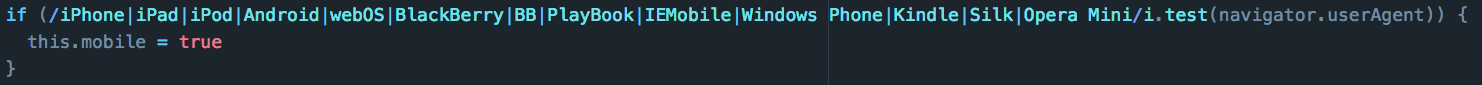
\includegraphics[width=7in]{./code/device_check.png}
	\caption{An if statement that checks to see if the device it is running on is a mobile or tablet}
\end{figure}

\begin{figure}[H]
	\centering
	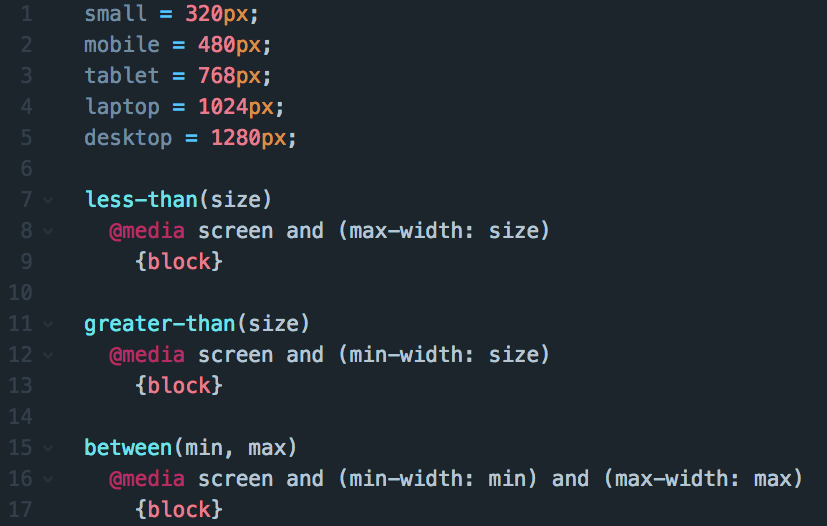
\includegraphics[scale=.3]{./code/breakpoints.png}
	\caption{Custom sylus code that defines breakpoints at common screen sizes from desktop to small mobile devices}
\end{figure}

\begin{figure}[H]
	\centering
	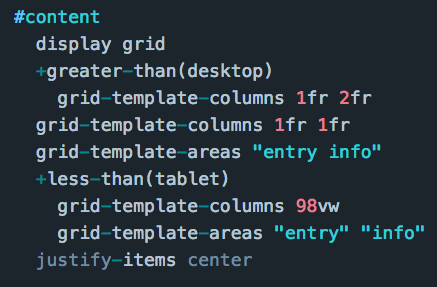
\includegraphics[scale=.3]{./code/breakpoints_example.png}
	\caption{An example of the breakpoints code being used to define how the page will react when sized greater than a desktop device or less than the size of a tablet}
\end{figure}

\begin{figure}[H]
	\centering
	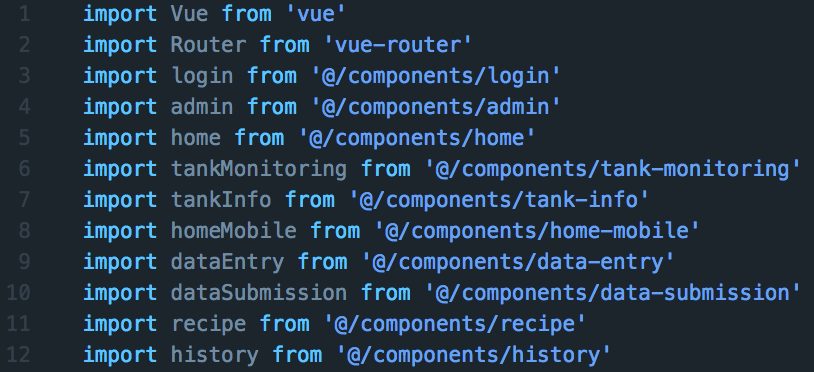
\includegraphics[scale=.3]{./code/routes_imports.png}
	\caption{The process of importing all the Vue components into the routes page so the router knows where to send the user to when they hit a certain path}
\end{figure}

\begin{figure}[H]
	\centering
	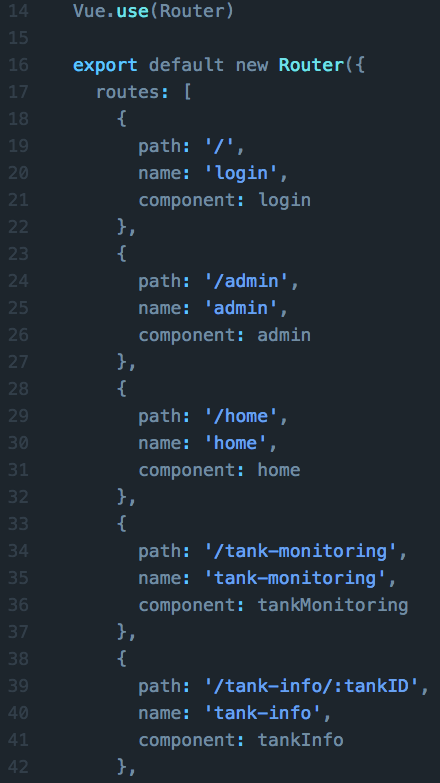
\includegraphics[scale=.3]{./code/routes.png}
	\caption{The mapping of url paths to components}
\end{figure}

\begin{figure}[H]
	\centering
	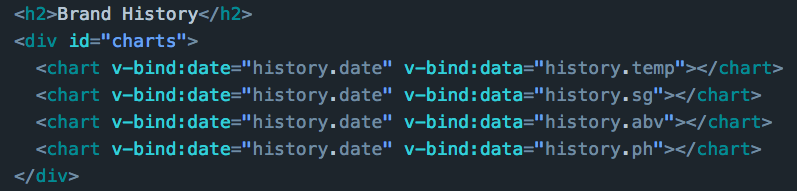
\includegraphics[scale=.3]{./code/components.png}
	\caption{A use of chart components on the tank-info page. Each chart has the dates and values passed into the component as a prop}
\end{figure}

\begin{figure}[H]
	\centering
	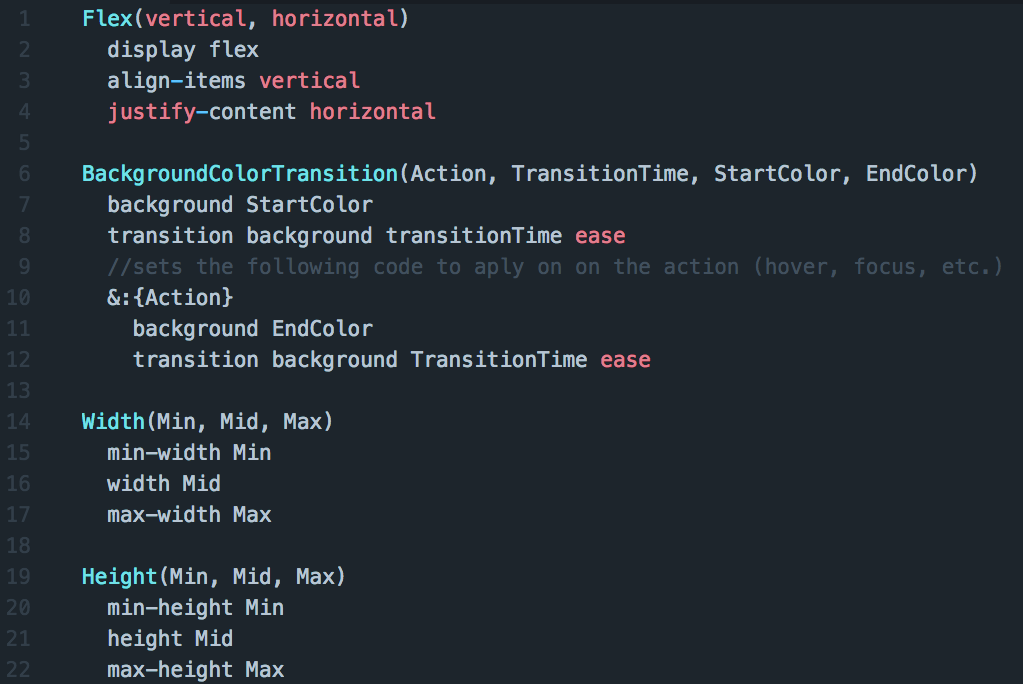
\includegraphics[scale=.3]{./code/mixins.png}
	\caption{Some additional custom Stylus functions to be used throughout the program to make the code easier to read and more modular}
\end{figure}

\section{Appendix 2: Additional Items}


\end{document}
